%%%%%%%%%%%%%%%%%%%%%%%%%%%%%%%%%%%%%%%%%%%%%%%%%%%%%%%%%%%%%%%%%%%%%%%%%%%%%%%%
% Preámbulo                                                                    %
%%%%%%%%%%%%%%%%%%%%%%%%%%%%%%%%%%%%%%%%%%%%%%%%%%%%%%%%%%%%%%%%%%%%%%%%%%%%%%%%

\RequirePackage{pdfmanagement-testphase}
\DeclareDocumentMetadata{pdfversion=2.0}

\documentclass[11pt,a4paper,titlepage,twoside,openright,openbib,spanish]{report}

%%% RELACIÓN DE VARIABLES A PERSONALIZAR %%%
\def\lingua{esp} % descomenta esta liña se redactarás a memoria en español
\def\nome{Alonso Rodríguez Iglesias}                             % substitúe aquí o teu nome
\def\nomedirectorA{Gabriel Rodríguez Álvarez}             % substitúe aquí o nome de quen dirixe
\def\nomedirectorB{Juan Touriño Domínguez}             % substitúe aquí o nome de quen dirixe
\def\titulo{Análisis del rendimiento de la inferencia de redes de aprendizaje profundo en arquitecturas de altas prestaciones} % substitúe aquí o título do teu TFM
% \def\mencion{ENXEÑARÍA DE COMPUTADORES}

\def\renomearcadros{si} % descomenta esta liña se redactas a memoria en español e prefires que
                         % os "cuadros" e o "índice de cuadros" se renomeen
                         % a "tablas" e "índice de tablas" respectivamente

\usepackage{estilo_tfm}

% Lista de paquetes potencialmente interesantes (uso baixo demanda)

\usepackage[all]{nowidow}
% \usepackage{alltt}       % proporciona o entorno alltt, semellante a verbatim pero que respecta comandos
% \usepackage{enumitem}    % permite personalizar os entornos de lista
% \usepackage{eurofont}    % proporciona o comando \euro
\usepackage{eurosym}
\usepackage{float}       % permite máis opcións para controlar obxectos flotantes (táboas, figuras)
\usepackage{hhline}      % permie personalizar as liñas horizontais en arrays e táboas
% \usepackage{longtable}   % permite construir táboas que ocupan máis dunha páxina
\usepackage{lscape}      % permite colocar partes do documento en orientación apaisada
% \usepackage{moreverb}    % permite personalizar o entorno verbatim
\usepackage{multirow}    % permite crear celdas que ocupan varias filas da mesma táboa
\usepackage{pdfpages}    % permite insertar ficheiros en PDF no documento
\usepackage{rotating}    % permite diferentes tipos de rotacións para figuras e táboas
% \usepackage{subcaption}  % permite a inclusión de varias subfiguras nunha figura
% \usepackage{tabu}        % permite táboas flexibles
% \usepackage{tabularx}    % permite táboas con columnas de anchura determinada
\usepackage{pdflscape}
\usepackage{translator}
\usepackage{placeins}
\usepackage{tablefootnote}

\usepackage[scale=MatchLowercase]{sourcecodepro}
\usepackage{pgfplots}
\usepackage{pgfgantt}
\newganttlinktype{F-S}{
  \ganttsetstartanchor{east}
  \ganttsetendanchor{west}
  \draw [/pgfgantt/link] (\xLeft - 0.2,\yUpper) -- (\xRight + 0.2, \yLower);
}

\newganttlinktype{F_S}{
  \ganttsetstartanchor{east}
  \ganttsetendanchor{west}
  \draw [/pgfgantt/link] (\xLeft - 0.2,\yUpper) |- (\xRight + 0.2, \yLower);
}

\newganttlinktype{S-S}{
  \ganttsetstartanchor{west}
  \ganttsetendanchor{west}
  \draw [/pgfgantt/link] (\xLeft + 0.2,\yUpper) |- (\xRight, \yLower);
}

\newganttlinktype{F-F}{
  \ganttsetstartanchor{east}
  \ganttsetendanchor{east}
  \draw [/pgfgantt/link] (\xLeft - 0.2 ,\yUpper) -| (\xRight - 0.2, \yLower);
}

\newganttlinktype{F-S}{
  \ganttsetstartanchor{east}
  \ganttsetendanchor{west}
  \draw [/pgfgantt/link] (\xLeft - 0.2,\yUpper) -| (\xRight + 0.2, \yLower);
}
\usepackage{pgfplotstable}
\pgfplotsset{compat = newest}
\usepackage{wrapfig}
\usepackage{etoolbox}
\BeforeBeginEnvironment{wrapfigure}{\setlength{\intextsep}{0pt}}
\usepackage{svg}
\usepackage{adjustbox}
\newcommand{\vasymptote}[2][]{
    \draw [thick,ficblue,densely dashed,#1] ({rel axis cs:0,0} -| {axis cs:#2,0}) -- ({rel axis cs:0,1} -| {axis cs:#2,0});
}
\pgfplotsset{every axis/.append style={
        scaled y ticks = false, 
        scaled x ticks = false, 
        y tick label style={/pgf/number format/.cd, fixed},
        x tick label style={/pgf/number format/.cd, fixed}
    }
}

%%%%%%%%%% Convenient math things
\newcommand{\pluseq}{\mathrel{+}=}
\newcommand{\asteq}{\mathrel{*}=}

%%%%%%%%%%%%%%%%%%%%%%%%%%%%%%%%%%%%%%%%%%%%%%%%%%%%%%%%%%%%%%%%%%%%%%%%%%%%%%%%
% Corpo                                                                        %
%%%%%%%%%%%%%%%%%%%%%%%%%%%%%%%%%%%%%%%%%%%%%%%%%%%%%%%%%%%%%%%%%%%%%%%%%%%%%%%%

\begin{document}

%%%%%%%%%%%%%%%%%%%%%%%%%%%%%%%%%%%%%%%%
% Preliminares do documento            %
%%%%%%%%%%%%%%%%%%%%%%%%%%%%%%%%%%%%%%%%

\begin{titlepage}
  
  \hspace*{128pt}
  \textcolor{udcgray}{{\fontencoding{T1}\fontfamily{phv}\selectfont Departamento de Ingeniería de Computadores}}\\[-2pt]
  \hspace*{145pt}
  \textcolor{udcpink}{{\fontencoding{T1}\fontfamily{phv}\selectfont Facultad de Informática de A Coruña}}\\[-32pt]

  \begin{center}
    
\includegraphics[scale=0.3]{img/udc.png}\\[35pt]

    {\large TRABAJO FIN DE MÁSTER \\
            MÁSTER INTERUNIVERSITARIO EN \\
            COMPUTACIÓN DE ALTAS PRESTACIONES } \\[100pt]
    
    \begin{huge}
      \begin{spacing}{1.3}
        \bfseries \titulo
      \end{spacing}
    \end{huge}
  \end{center}
  
  \vfill
  
  \begin{flushright}
    {\large
    \begin{tabular}{ll}
      {\bf Estudiante:} & \nome \\
      {\bf Directores:} & \nomedirectorA \\ % COPIA E PEGA ESTA LIÑA MÁIS VECES SE O PRECISAS
                        & \nomedirectorB \\ % COPIA E PEGA ESTA LIÑA MÁIS VECES SE O PRECISAS
    \end{tabular}}
  \end{flushright}
  \rightline{A Coruña, \today}
\end{titlepage}

\paxinaenbranco
\begin{flushright}
\dedicatoria{A todas las personas que me apoyaron en los buenos y los malos momentos.\\Gracias a ellos hoy soy quien soy.}
\end{flushright}
\paxinaenbranco
\paxinaenbranco
\begin{agradecementos}
A Gabriel y Juan por darme esta oportunidad, a mis amigos y seres queridos, que han hecho un poco más sobrellevable este (otra vez) atípico año, no solo apoyándome siempre en mis objetivos, sino también personalmente, y especialmente a Xián por su inestimable ayuda con el domado de la pitón.

Muchas gracias.

\begin{flushright}
Alonso
\end{flushright}
\end{agradecementos}
% Ugly hack to fix random pagenumber %%%%%%
\pagenumbering{gobble}
\pagestyle{empty}
%%%%%%%%%%%%%%%%%%%%%%%%%%%%%%%%%%%%%%%%%%%
\paxinaenbranco
%%%%%%%%%%%%%%%%%%%%%%%%%%%%%%%%%%%%%%%%%%%%%%%%%%%%%%%%%%%%%%%%%%%%%%%%%%%%%%%%
\begin{abstract}\thispagestyle{empty}
  En un mundo donde la inteligencia artificial es cada vez más atractiva para el público general, con modelos que realizan tareas como la conducción autónoma, se puede ver cómo estas redes neuronales, que llevan evolucionando a enorme velocidad los últimos años, son cada vez más útiles en la sociedad actual, generándose así una gran demanda computacional y energética tanto en los dispositivos más grandes, como los automóviles, como en los más pequeños, como pulseras inteligentes. Debido a esta razón, cada vez son más necesarias arquitecturas de altas prestaciones y elevada eficiencia energética para optimizar su rendimiento.

  Este Trabajo Fin de Máster se centra en el análisis, mejora y medida del rendimiento de ejecución de modelos de inteligencia artificial con redes \textit{feed-forward} dispersas en fase de inferencia. Mediante el uso de una herramienta para generación de código C desde modelos TensorFlow se comparan diferentes aproximaciones a la multiplicación de matrices, clave en inteligencia artificial, y se allana el camino hacia subsiguientes optimizaciones.

  \vspace*{22pt}
  \begin{segundoresumo}
  \vspace*{-3pt}

  In a world where artificial intelligence is becoming increasingly attractive to the general public, with models performing tasks such as autonomous driving, we can see how these neural networks, which have been evolving at enormous speed in recent years, are becoming increasingly useful in the current society, thus generating a high computational and energy demand in both larger devices, such as cars, and smaller ones, such as smart bands. For this reason, high performance and efficient architectures are increasingly necessary to optimize their performance.

  This dissertation focuses on the analysis, improvement and execution performance measurement of artificial intelligence models with sparse \textit{feed-forward} networks in the inference phase. By using a tool for C code generation from TensorFlow models, we compare different approaches to matrix multiplication, key in artificial intelligence, and pave the way to subsequent optimizations.

  \end{segundoresumo}
\vspace*{25pt}
\begin{multicols}{2}
\begin{description}
\item [\palabraschaveprincipal:] \mbox{} \\[-20pt]
  \begin{itemize}
    \item Redes Neuronales
    \item High Performance Computing
    \item Computación Dispersa
    \item Generación de Código
  \end{itemize}
\end{description}
\begin{description}
\item [\palabraschavesecundaria:] \mbox{} \\[-20pt]
  \begin{itemize}
    \item Neural Networks
    \item High Performance Computing
    \item Sparse Computation
    \item Code Generation
  \end{itemize}
\end{description}
\end{multicols}
\end{abstract}
%%%%%%%%%%%%%%%%%%%%%%%%%%%%%%%%%%%%%%%%%%%%%%%%%%%%%%%%%%%%%%%%%%%%%%%%%%%%%%%%
%\paxinaenbranco
%Restore thinges %%%
\pagestyle{fancy}
%%%%%%%%%%%%%%%%%%%%

\pagenumbering{roman}
\setcounter{page}{1}
\bstctlcite{IEEEexample:BSTcontrol}

\tableofcontents
\listoffigures
\listoftables
\cleardoublepage

\pagenumbering{arabic}
\setcounter{page}{1}

%%%%%%%%%%%%%%%%%%%%%%%%%%%%%%%%%%%%%%%%
% Capítulos                            %
%%%%%%%%%%%%%%%%%%%%%%%%%%%%%%%%%%%%%%%%

\chapter{Introducción}
\label{chap:introducion}

\lettrine{E}{n} este capítulo se expondrá qué motivó este trabajo y sus objetivos, así como qué estructura seguirá la memoria del mismo.

%Ejemplo: capítulo da memoria, onde xeralmente se exporán as
%liñas mestras do traballo, os obxectivos, etc. Incluimos un par de
%exemplos de citas~\cite{ErlangBook,ErlangWebBook} e de referencias
%internas (sección \ref{sec:mostra}, páxina \pageref{sec:mostra}).

\section{Motivación}
\label{sec:motivacion}

La computación de altas prestaciones (\acrshort{hpc}, \acrlong{hpc}) y la inteligencia artificial (\acrshort{ia}) están de moda. Quizás más la segunda que la primera, pero lo cierto es que, sin base sobre la que ejecutarse, la segunda no tiene mucho que hacer.
Los supercomputadores son equipos informáticos compuestos por miles de procesadores, así como cantidades ingentes de memoria para ofrecer una elevada capacidad y velocidad de cálculo y procesamiento de datos.
Sin embargo, estas máquinas y sus mecanismos y procesos tan potentes suelen quedar muchas veces fuera de la comprensión no solo del público general, sino incluso de las personas que tienen la informática como \textit{hobby} o profesión.

Para no quedarse atrás, la Unión Europea está realizando una muy importante inversión en las dos disciplinas anterioremente mencionadas, pero especialmente en \acrshort{hpc}, donde la inversión ya supera a la de la \acrshort{ia}, como se puede ver en una hoja publicada por la Unión Europea en \cite{eu_factsheet_digital}.
Por esta razón, este \acrshort{tfg} tiene como objetivo atraer la atención de futuros ingenieros hacia este sector clave, que tanta inversión recibe y se espera que siga recibiendo. Para ello se construirá un pequeño clúster con Raspberry Pis con el nombre de Clúpiter, con el que poder realizar explicaciones acerca de cómo funciona este tan apasionante y demandado ámbito de la informática.

El principal componente de Clúpiter, la Raspberry Pi, es un computador de formato muy reducido y bajo consumo y coste, usado muy habitualmente en proyectos amateur y entornos educativos, lo que posibilita su empleo en proyectos de divulgación como el que aquí se realiza.

\section{Objetivos}
\label{sec:objetivos}

El principal objetivo de este trabajo es acercar la supercomputación y el procesamiento paralelo a públicos no especializados de una forma didáctica y amena mediante la construcción de un clúster que pueda emular el funcionamiento de un supercomputador. Para conseguir este objetivo primero necesitaremos una base tangible con la que trabajar y sobre la que podamos realizar las explicaciones. Esto es, el hardware del clúster, que se construirá utilizando las previamente mencionadas Raspberry Pis. El sistema construido pretende ser una réplica a pequeña escala de los supercomputadores actuales.

Sobre este hardware debe correr un sistema operativo en el que ejecutar los benchmarks y demostraciones, tanto a efectos académicos como divulgativos, respectivamente. Este sistema operativo será Arch Linux, un Linux que se define como ``una distribución ligera y flexible que intenta mantener la simplicidad'', y que sigue los principios de Simplicidad, Modernidad, Pragmatismo, Centralidad del Usuario y Versatilidad\footnote{\url{https://wiki.archlinux.org/title/Arch\_Linux}}.

En el transcurso del proyecto se conectarán y configurarán las Raspberry Pi para que puedan trabajar de forma colaborativa como si se tratase de un único equipo, permitiendo así realizar divulgación acerca del \acrshort{hpc} a alumnos de secundaria y bachillerato que tengan interés en la carrera, así como también al público general.

Asimismo, la base hardware y software también debe servir para futuros TFGs que mejoren o amplíen ciertas características de Clúpiter, como su mantenibilidad, seguridad, características de alta disponibilidad, etc, siendo estas de nuevo habilidades muy demandadas por la Unión Europea y que están sujetas a fuertes inversiones actuales y futuras.



\section{Estructura}
\label{sec:estructura}
Esta memoria describe el proceso de desarrollo de Clúpiter, siguiendo un esquema relacionado con el ciclo de vida del mismo, el incremental.

De esta forma, primero se da una introducción y los conceptos básicos del proyecto. Tras ello, se describe el proceso de codiseño hardware y software siguiendo las etapas del ciclo de vida, que son análisis, diseño, implementación y pruebas.

Tras esto, se detalla la creación de la aplicación web (el \textit{dashboard}), también desglosado en sus diferentes fases, ya que se considera un elemento lo suficientemente diferenciado como para no incluirlo en el ciclo de vida general.

En el penúltimo capítulo se muestra la planificación y los hipotéticos costes derivados de las horas invertidas en este proyecto, así como los costes reales del hardware adquirido. Tras ello, se muestran las conclusiones sacadas a lo largo del proyecto, la relación con la titulación en cuanto a las disciplinas requeridas para la realización del mismo, y se proponen líneas de trabajo futuras en forma de ideas para nuevas iteraciones sobre esta plataforma. 

\chapter{Conceptos básicos}
\label{chap:conceptos_basicos}

\lettrine{P}{ara} una correcta comprensión de los objetivos de este trabajo, tanto a corto como a largo plazo, es necesario poseer una serie de conceptos básicos relacionados con las redes neuronales, su estructura, rendimiento y cómo se implementan en un procesador moderno, para posteriormente poder comprender las mejoras propuestas a continuación.

\section{Redes neuronales}
\label{sec:redes_neuronales}
Las redes neuronales constituyen la base de la mayoría de los últimos avances en el campo de la inteligencia artificial. A pesar de la enorme diversidad en \textit{layouts} de capas, neuronas, funciones de transferencia, etc., la realidad es que el álgebra lineal y la multiplicación de matrices son parte fundamental e imprescindible para la ejecución de las mismas \cite[Figura 3.4]{deep_learning_for_computer_architects}.

A pesar de que en la Prueba de Concepto (\acrlong{poc} o \acrshort{poc} por sus siglas en inglés) expuesta en el Capítulo \ref{chap:desarrollo_poc} se trabaja únicamente con redes \textit{feed-forward}, sería naíf pensar que solamente existen estas arquitecturas de redes neuronales. Ejemplos a destacar pueden ser las redes convolucionales, empleadas principalmente para el procesado de imágenes, las basadas en modelos secuenciales o en transformers, que están revolucionando el mundo de la inteligencia artificial mediante modelos de procesamiento del lenguaje o de generación de imágenes, así como muchas otras como las redes GAN, o las basadas en arquitecturas \textit{encoder-decoder}.

Estas arquitecturas son llamadas de redes neuronales, a pesar de que, como es evidente, una neurona no puede como tal ``ejecutar'' una convolución. Más bien, estas nuevas arquitecturas se basan en la modelación de operaciones matemáticas complejas en pasos discretos, como por ejemplo la convolución anteriormente mencionada.

\subsection{Estructura de una red neuronal \textit{feed-forward}}
\label{ssec:estructura_red_neuronal_ff}
Las redes neuronales \textit{feed-forward} se componen de varias capas de neuronas que toman una o más entradas, realizan la suma de todas ellas, suman un \textit{bias}, y finalmente aplican una función de transferencia no lineal.

La capa que toma los datos de entrada se llama capa \textit{input} o de entrada, y la capa que expulsa los datos de salida es la capa \textit{output} o de salida. Las capas que realizan transformaciones intermedias se denominan capas ocultas o \textit{hidden layers}.

En la Figura \ref{fig:dense_nn_sample}\footnote{Imagen generada con la herramienta NN-SVG, disponible en \url{https://alexlenail.me/NN-SVG}} se puede ver un diagrama de una red neuronal \textit{feed-forward} densa. Esto es, una red neuronal en la que cada neurona de una capa está conectada con todas las neuronas de la capa siguiente. Esto se traduce en que la matriz de pesos que representa cada capa es una matriz densa, o dicho de otra manera, que no contiene pesos con valor cero.

\begin{figure}[h!]
    \centering
    \vspace*{0.5cm}
    \def\svgwidth{0.85\textwidth}
    \input{pdf_tex/dense_nn/dense_nn_svgnn.pdf_tex}
    \caption{Red neuronal densa \textit{feed-forward}}
    \label{fig:dense_nn_sample}
\end{figure}

Por el contrario, como se puede ver en la Figura \ref{fig:sparse_nn_sample}, existen las redes neuronales dispersas, en las que una cantidad significativa de los pesos tienen valor cero. Estas redes se pueden obtener de múltiples formas, y sus objetivos son variados, a pesar de que el principal objetivo es reducir el tamaño del modelo.

Uno de los posibles métodos para la obtención de una red neuronal dispersa (\textit{sparse}) es mediante el podado o \textit{pruning}. Este método, sorprendentemente similar al empleado por neurocirujanos durante operaciones a cerebro abierto, consiste en ir cortando conexiones de forma más o menos arbitraria (en función del algoritmo) y observando cómo varía la salida. En caso de que la salida sea correcta, se continúa en esa dirección. Para que un cambio en una red neuronal se considere inapreciable, la salida debe verse alterada de tal forma que sea indistinguible su efecto del de unos diferentes parámetros iniciales durante el entrenamiento, lo cual implica que será corregible mediante un reentrenamiento. Esta variación se mide con la métrica \textit{\acrlong{itn}} o \acrshort{itn} \cite[4.1.1]{deep_learning_for_computer_architects}.

De esta forma, una red neuronal dispersa puede contener alrededor de un 80-90\% menos de conexiones entre neuronas, representando esto un ahorro sustancial de energía en términos de acceso a memoria, relevante en sistemas miniaturizados donde cada milivatio cuenta.

\begin{figure}[h!]
    \centering
    \vspace*{0.5cm}
    \def\svgwidth{0.85\textwidth}
    \input{pdf_tex/sparse_nn/sparse_nn_svgnn.pdf_tex}
    \caption{Red neuronal dispersa \textit{feed-forward}}
    \label{fig:sparse_nn_sample}
\end{figure}

Esta operación de podado puede no solamente limitarse a los pesos que interconectan neuronas, sino que se puede hacer el modelo más eficiente y reducido al podar todos los pesos entrantes en una neurona, eliminando por completo dicha neurona, y por tanto eliminando también todas sus conexiones posteriores en cadena. El efecto de eliminar una neurona sin conexiones entrantes, que únicamente arroja valores constantes en cada iteración, se puede compensar ajustando el \textit{bias} del receptor que correspondía a esa neurona en las conexiones posteriores.

\subsection{Redes neuronales profundas}
\label{ssec:redes_reuronales_profundas}
El \textit{boom} de la inteligencia artificial en los últimos años viene dado en gran medida por el enorme crecimiento que ha experimentado el campo mediante técnicas de \textit{deep learning}, precisamente en estas redes neuronales profundas o \textit{deep neural networks}.

Y es que dentro de las infinitas posibilidades que nos ofrecen las neuronas artificiales tratadas anteriormente, existe la posibilidad de apilar capa sobre capa, obteniendo con cada capa extra comportamientos y patrones más complejos.
Es precisamente este comportamiento de los sistemas no lineales el que permite reproducir comportamientos exóticos al aumentar el número de neuronas y/o capas (y por tanto la complejidad) del sistema.

Tras sospechas previas de algunos investigadores como George Cybenko acerca de que una red neuronal con al menos una capa oculta es un aproximador universal, y tras demostrar dicho comportamiento para la sigmoide como función de transferencia \cite{cybenko1989approximation}, Kurt Hornik demostró en 1991 que una red neuronal de con al menos una capa oculta es siempre un aproximador universal, independientemente de la función de transferencia, siempre que esta sea no polinomial. A pesar de que una red neuronal de una sola capa oculta pueda ser un aproximador universal, se obtienen aproximaciones mucho más inteligentes y ``económicas'' computacionalmente al contar con más de una capa oculta \cite{hornik1991approximation}, donde el máximo exponente de esta doctrina es precisamente el \textit{deep learning}.

\section{Redes neuronales densas}
\label{sec:redes_reuronales_densas}
Como se comentó en la sección anterior, independientemente del número de capas de la red, sea profunda o ``convencional'', una red neuronal densa es aquella en la que para $m$ neuronas en la capa $M$, y $n$ neuronas en la capa $N$, donde la neurona $x$ de la capa $M$ se denota $M_{x}$, existe siempre una conexión de $M_{m}$ a $N_{n}$, es decir ($m\longrightarrow n$):

\begin{equation}
\forall m \in M \:\wedge\: \forall n \in N, \: m\longrightarrow n\nonumber
\label{eq:dense_nn}
\end{equation}

De esta forma, para la ejecución (inferencia) de una red neuronal densa \textit{feed-forward}, serán necesarias únicamente una simple multiplicación de matrices, una suma de matrices para tener en cuenta los \textit{bias}, y la aplicación de una función de transferencia.

Esto se puede apreciar en la Figura \ref{fig:nn_matrix_dense}\footnote{Imágenes con este estilo se han obtenido y modificado de \url{https://ml-cheatsheet.readthedocs.io/en/latest/forwardpropagation.html}}. En ella se puede ver el procesod de inferencia de 4 datos bidimensionales, correspondientes con el número de filas de entrada a las capas. Como también se puede apreciar, la anchura de cada capa se corresponde con el número de columnas de la misma. 

\begin{figure}[h!]
    \centering
    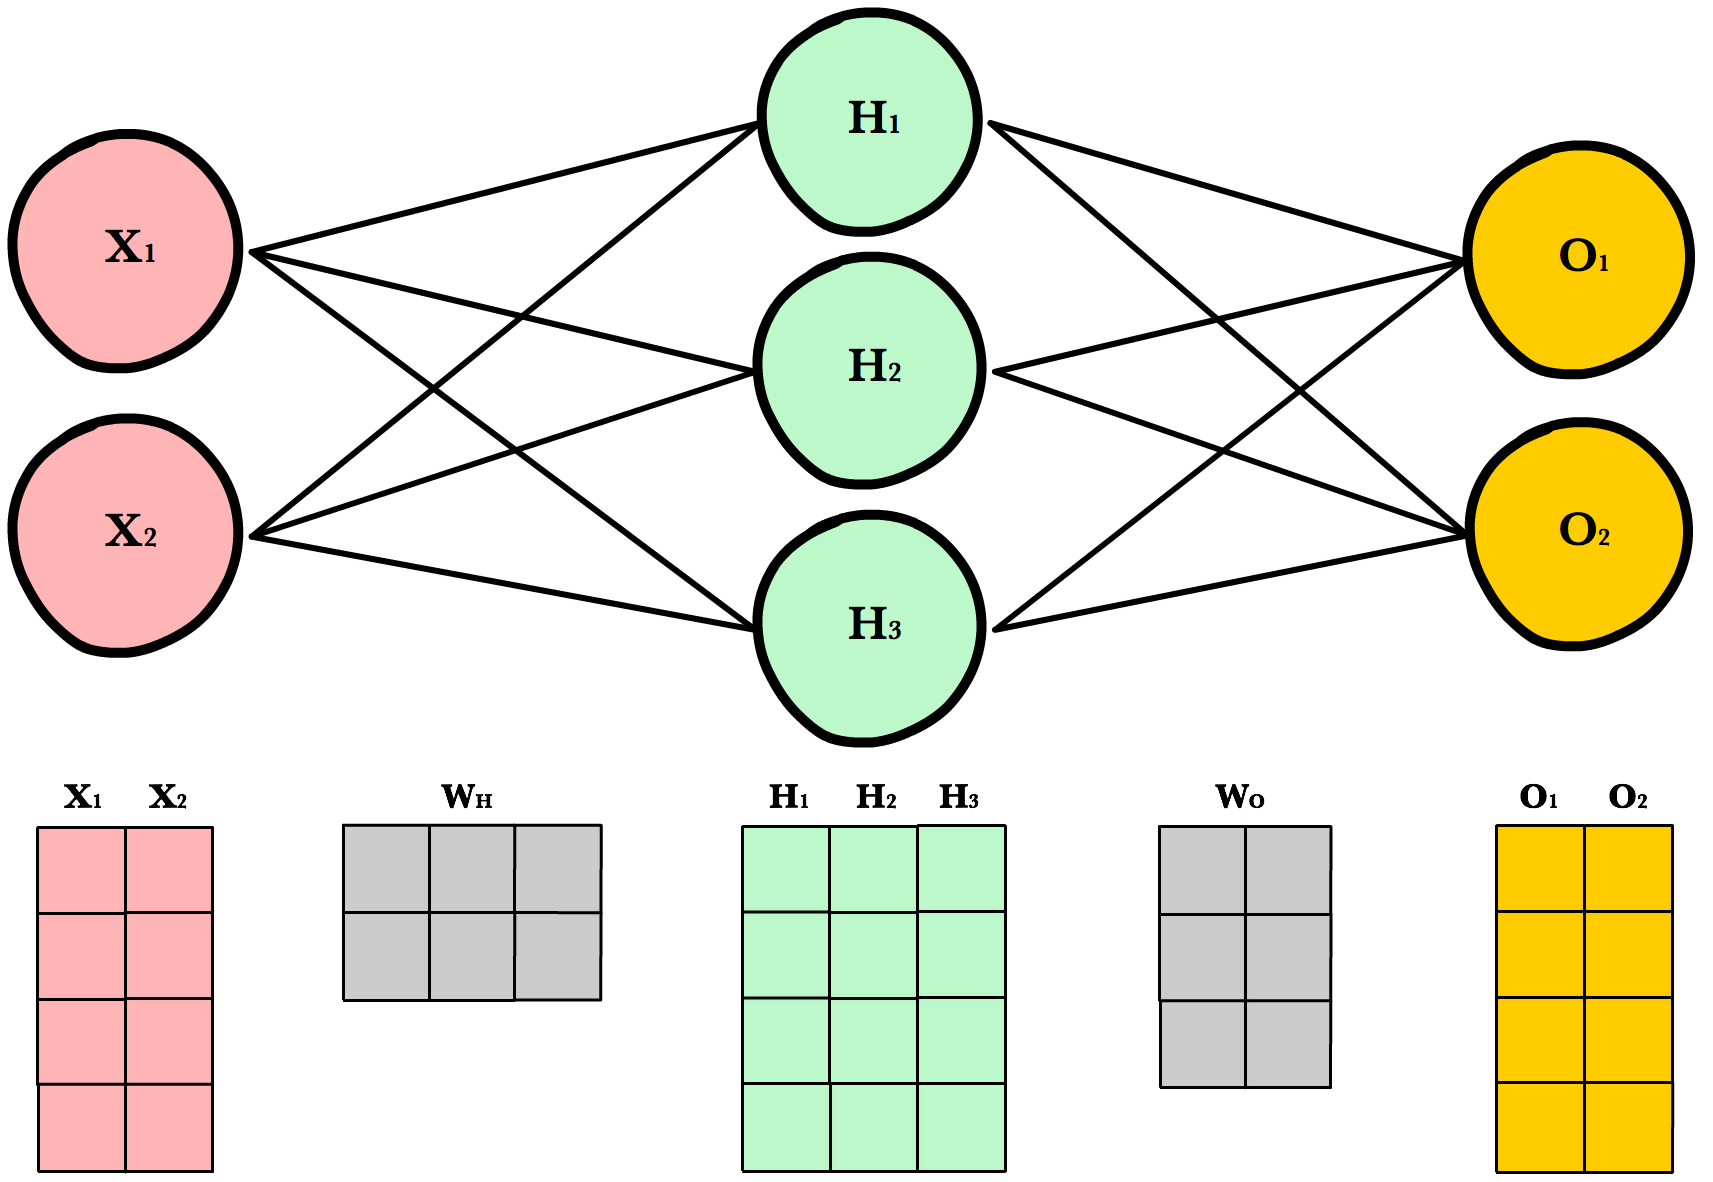
\includegraphics[width=0.85\textwidth]{img/neural_network_matrix_dense.png}
    \caption{Visualización de inferencia en redes neuronales densas}
    \label{fig:nn_matrix_dense}
\end{figure}

Así, si el dato (vectorial por la naturaleza de estas redes) tiene 24 elementos, será necesaria una capa de entrada de 24 neuronas (24 columnas $x_{1} .. x_{24}$ según notación de la Figura \ref{fig:nn_matrix_dense}), y si queremos inferir sobre 1000 de estos datos, esto se puede hacer en una sola ejecución, siendo el número de columnas también de 1000.

O dicho de otra manera, sea la capa $M_{m}$ una capa completamente conexa con $m$ neuronas, a la cual se le introduce un dato $x_{m}$, donde el peso de la neurona $M_{i}$ hacia $N_{j}$ se denota como $w_{M,i,j}$, y la función de transferencia es $\phi$, entonces se tiene que la salida de una capa será:

\begin{equation}
    x_{N,i} = \phi\left(\sum_{j}w_{N,i,j}x_{M,j}\right)\nonumber
    \label{eq:dense_nn_eq}
\end{equation}

A esta función se le puede añadir el \textit{bias} de forma explícita ($\sum\left([\dots] x_{M,j}\right) + bias_{N,i}$), o de forma implícita, siendo el \textit{bias} una conexión más, con un valor constante de 1, cuyo peso es el multiplicador que da el \textit{bias} resultante.

\section{Redes neuronales dispersas}
\label{sec:redes_reuronales_dispersas}
Las redes neuronales dispersas cuentan con una ventaja, y es el menor número de conexiones entre neuronas, o directamente el menor número de neuronas en la arquitectura. A pesar de esto, en realidad el fundamento matemático es el mismo, una simple multiplicación de matrices. Sin embargo, a pesar de tener el mismo funcionamiento base, se pueden explotar ciertas características, tanto de la estructura de las matrices dispersas como de su multiplicación, para obtener mejoras tanto en el tamaño del modelo como en su rendimiento, respectivamente.

\subsection{Fundamentos de matrices dispersas}
\label{ssec:fundamentos_matrices_dispersas}
Una matriz es dispersa cuando gran parte de su contenido son únicamente ceros. El cuan dispersa es una matriz se cuantifica mediante el ``grado de dispersión'' o \textit{sparsity}. Una matriz dispersa $10 \times 10$ con tres elementos diferentes de cero (denominados elementos \textit{nonzero} o directamente \textit{nonzeros}) será una matriz dispersa con una \textit{sparsity} del $97\%$ y una densidad del $3\% \:(=100\%-97\%)$.

\subsection{Almacenamiento de matrices dispersas}
\label{ssec:almacenamiento_matrices_dispersas}
Existen múltiples métodos para el almacenamiento de matrices dispersas en memoria, pero uno de los más sencillos de comprender, y que se usa en la \acrshort{poc} para la creación de las matrices dispersas, es el formato \acrshort{coo} o \textit{\acrlong{coo}}.

Este formato consiste en el almacenamiento de dato y coordenadas en tres vectores: \texttt{V}, \texttt{C} y \texttt{R} (\textit{Value}, \textit{Column}, \textit{Row}). Para cada entrada en el vector \texttt{V}, se crea una entrada en la misma posición para los vectores \texttt{C} y \texttt{R}, indicando la columna y fila en la que se ubica el valor \textit{nonzero}. Por diseño, el tamaño de cada uno de estos tres vectores tiene que ser igual al número de \textit{nonzeros}, denotado por \texttt{NZ}. Este formato es particularmente cómodo para la creación de matrices dispersas de forma ágil, pero existen formatos más avanzados, tanto en tamaño como en eficiencia, como el \acrshort{csr} o \textit{\acrlong{csr}}\footnote{Más información en \url{https://en.wikipedia.org/wiki/Sparse_matrix\#Compressed_sparse_row_(CSR,\_CRS\_or\_Yale\_format)}}.

A continuación se muestra un ejemplo de una matriz dispersa almacenada en formato \acrshort{coo}. A pesar de que esta matriz no es particularmente dispersa, se utiliza únicamente con fines explicativos:

\begin{center}
    $\begin{pmatrix}
        1 & 0 & 0 & 0\\
        0 & 2 & 0 & 0\\
        0 & 3 & 4 & 0\\
        0 & 0 & 0 & 5
    \end{pmatrix}$
    \vspace*{0.5cm}
\begin{lstlisting}[]
NZ = 5

V = [ 1 2 3 4 5 ]
C = [ 0 1 1 2 3 ]
R = [ 0 1 2 2 3 ]
\end{lstlisting}
\end{center}

\subsection{Propiedades del producto de matrices dispersas}
\label{ssec:propiedades_producto_matrices_dispersas}
Al multiplicar dos matrices densas no hay duda de que como resultado se obtendrá una matriz densa, salvo contadas excepciones, como multiplicar una matriz por su inversa. Sabiendo que el producto de matrices dispersas obtiene el mismo resultado que una multiplicación de matrices densas mediante un algoritmo diferente, se pueden clasificar los productos de matrices en función de su \textit{sparsity} de forma genérica.

Esta clasificación, de nuevo, puede variar en función de las propiedades de la matriz, pero es la base sobre la cual se construyen las funciones de \acrshort{blas} (\textit{\acrlong{blas}}) \cite{netlib_blas} y las implementaciones Sparse BLAS \cite{sparse_blas_10.1145/567806.567810}. De esta forma, se pueden implementar los siguientes tipos de producto de matrices:

\begin{itemize}
    \item Densa $\times$ Densa $=$ Densa ($D\times D$)
    \item Dispersa $\times$ Densa $=$ Densa ($d\times D$)
    \item Dispersa $\times$ Dispersa $=$ Dispersa / Densa\footnote{En función de la forma en que los valores \textit{nonzero} estén dispuestos en ambas matrices, el resultado puede ser una matriz dispersa o densa.} ($d\times d$)
\end{itemize}

Estos tres tipos principales de productos, en típico \textit{BLAS-fashion} se pueden realizar para tipos de datos según su precisión, \texttt{S}, \texttt{D}, \texttt{C} y \texttt{Z} (\textit{Single}, \textit{Double}, \textit{Single Complex}, \textit{Double Complex}).
Así, se pueden obtener las siguientes funciones estándar, a pesar de que en la parte \textit{sparse} de \acrshort{blas} hay menor consenso debido a la existencia de múltiples librerías que difieren del estándar por ser previas a la creación del mismo. Por ejemplo, los tipos especificados en la función se van perdiendo conforme se avanza hacia implementaciones genéricas en C++.

\begin{itemize}
    \item \texttt{[sdcz]gemm()} para $D\times D$
    \item \texttt{[sdcz]usmm()} o \texttt{spmm()} para $d\times D$
    \item \texttt{sp[sdcz]gemm()} o \texttt{spmsp()} para $d\times d$
\end{itemize}

Sabiendo las características de una red neuronal dispersa, y tal como se comenta más adelante en esta memoria, en la \acrshort{poc} se emplea el producto $d\times D$, debido a la naturaleza dispersa de los pesos, y densa de los datos de entrada. De todas formas, en función de la naturaleza de los datos de entrada, podrían emplearse también vectores de entrada dispersos, aunque lo más probable es que para eso quizás una red neuronal \textit{feed-forward} unidimensional no sea lo más apropiado, y ya se deban sugerir otras arquitecturas de red como las convolucionales, debido a que un vector disperso no suele tener mucho sentido, pero una matriz dispersa sí.
x
\subsection{Visualización de una red neuronal dispersa}
\label{ssec:visualizacion_nn_dispersa}
Tal como se mostró en la Sección \ref{sec:redes_reuronales_densas}, es sencillo visualizar el proceso de inferencia como una simple multiplicación de matrices, por lo que una multiplicación con una matriz de pesos dispersa debería ser sencilla de visualizar de forma similar.

Y este razonamiento es correcto, es muy sencilla de visualizar de no ser por un pequeño detalle. Y es que la función de multiplicación de matrices $d\times D$, \texttt{[sdcz]usmm()}, tiene una firma poco genérica, haciendo que, si bien esta función parezca adecuada para esta carga de trabajo, tenga un sutil detalle que requiere un poco de detenimiento. A continuación se muestra para el lenguaje C y para simple precisión la firma y parámetros de la función \texttt{BLAS\_susmm}:

\begin{lstlisting}[language=C]
int BLAS_susmm( enum blas_order_type    order,
                enum blas_trans_type    transA,
                int                     nrhs,
                float                   alpha,
                blas_sparse_matrix      A,
                const float *           b,
                int                     ldb,
                float *                 c,
                int                     ldc 
)

/**
 * order    Layout of the dense array.
 * transA   Transposition operator for matrix A.
 * nrhs     Number of right hand side columns.
 * A        A valid matrix handle.
 * alpha    Value for alpha.
 * b        Dense vector b.
 * ldb      Leading dimension of b.
 * c        Dense vector c.
 * ldc      Leading dimension of c.
 */
\end{lstlisting}

El inconveniente de esta función, que calcula $C = \alpha AB + C$, es que la matriz $A$ debe ser dispersa, algo que, fijándose de nuevo en la Figura \ref{fig:nn_matrix_dense}, no se cumple. Es decir, la matriz dispersa es la de pesos $w$, por lo que parece necesaria una función que trate a $B$ como una matriz dispersa. Dicha función no existe.

\begin{figure}[h!]
    \centering
    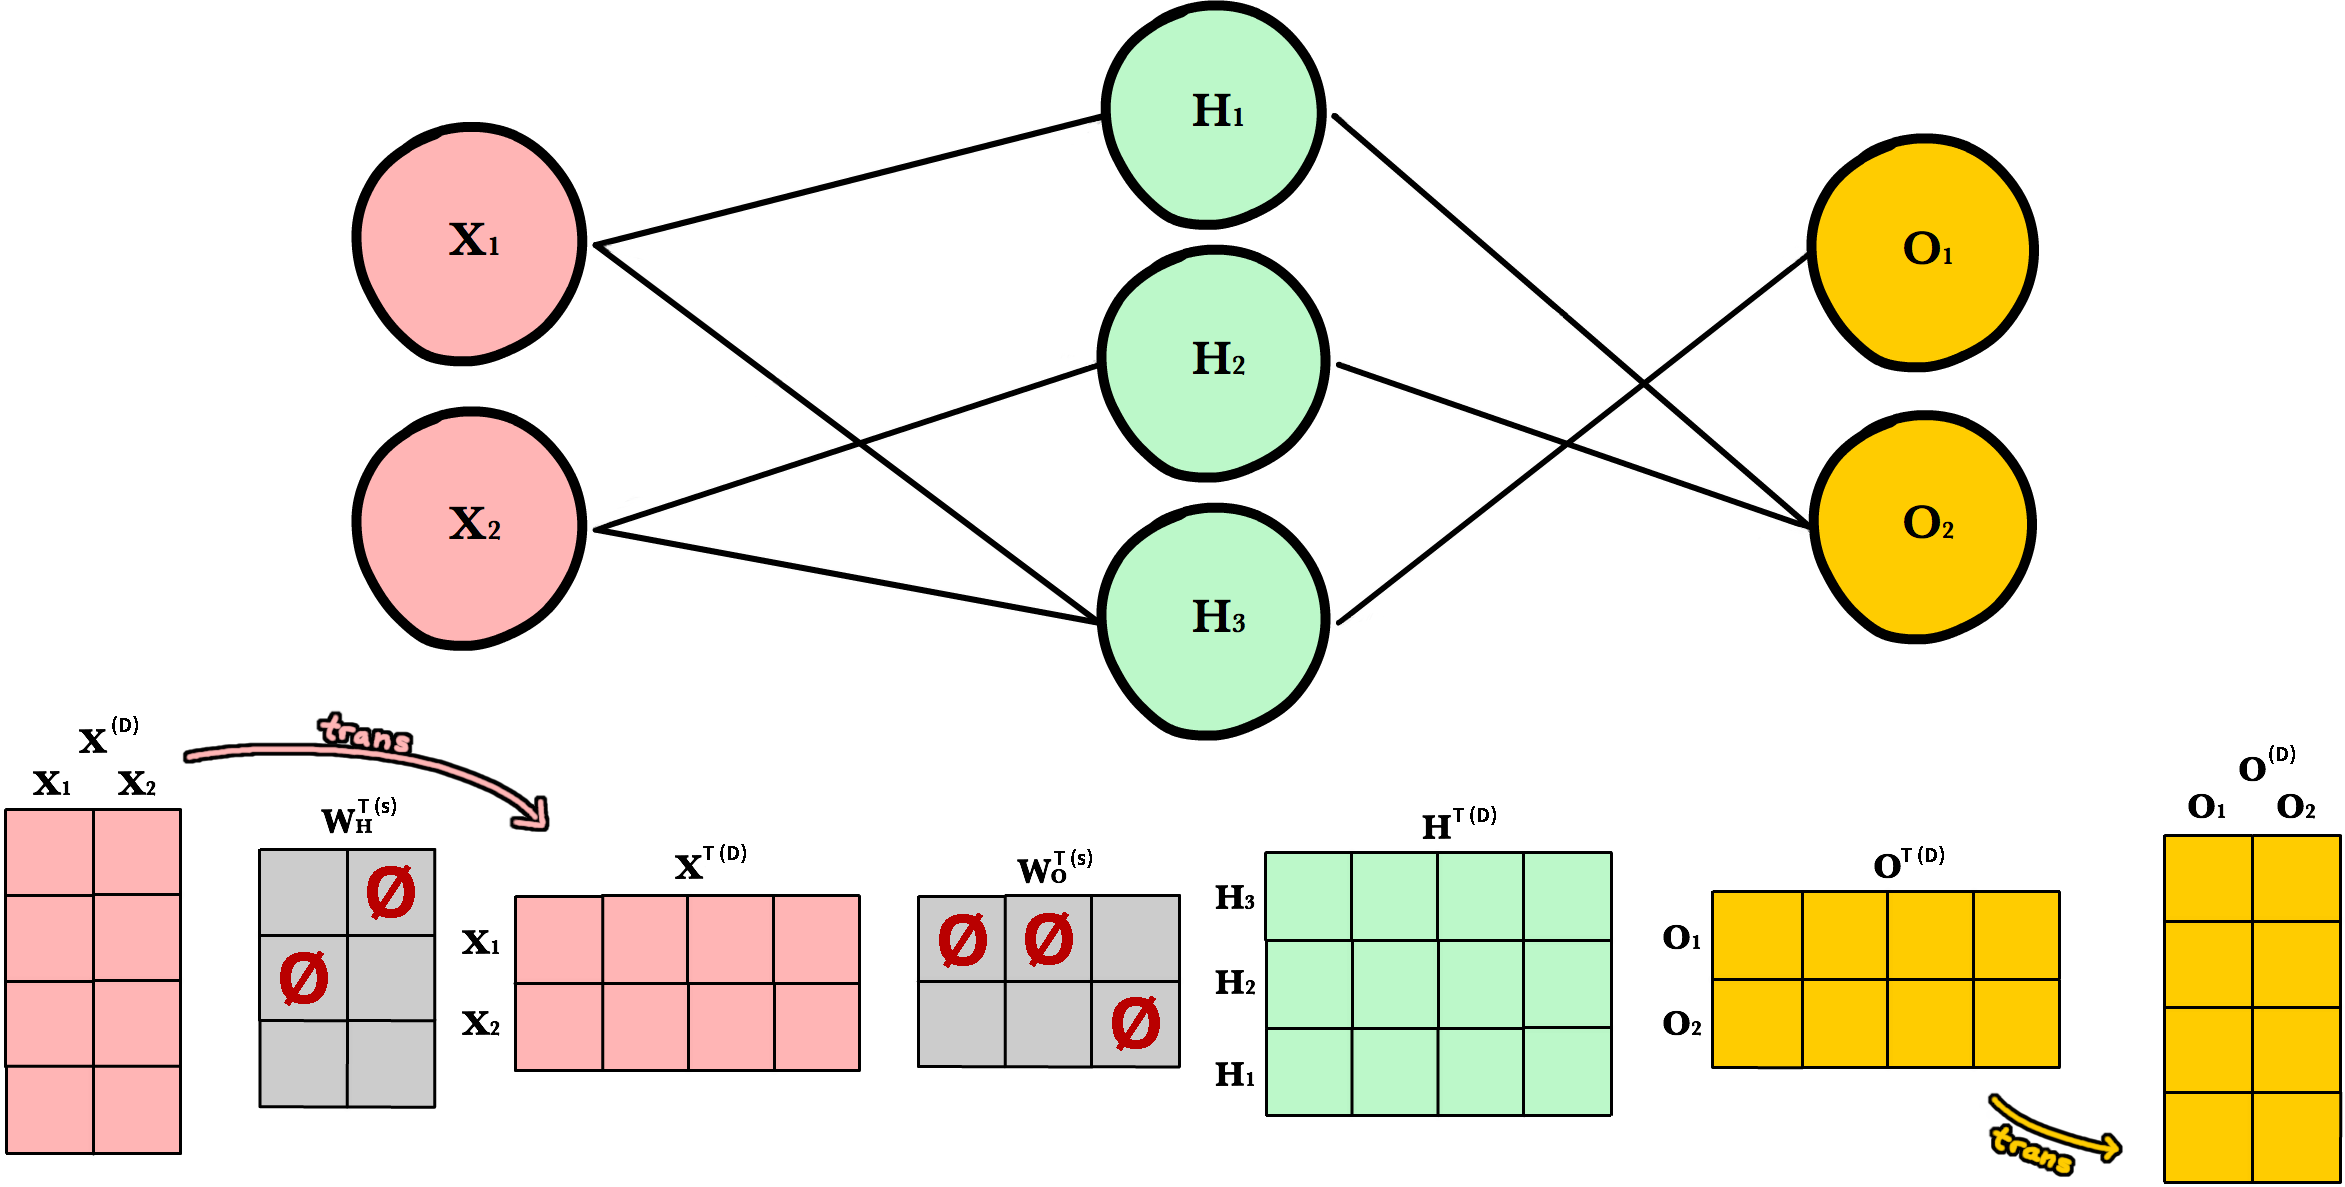
\includegraphics[width=\textwidth]{img/neural_network_matrix_sparse/neural_network_matrix_sparse.png}
    \caption{Visualización de inferencia en redes neuronales dispersas}
    \label{fig:nn_matrix_sparse}
\end{figure}

Sin embargo, empleando las propiedades de las matrices, es posible modificar el orden de las mismas, y así poder encajar cada matriz en la firma. Para esto se emplea una propiedad básica de las matrices, $C^{T} = (AB)^{T} = A^{T}B^{T}$. De esta forma, al transponer la matriz de pesos mediante el parámetro \texttt{transA}, y multiplicando esto por la salida de la capa anterior, se obtiene la salida $C^{T}$. Esto supone un pequeño overhead, al tener que transponer la entrada a la capa de entrada, así como la salida de la capa de salida. Sin embargo, dicho overhead puede mitigarse en gran medida, en función de la arquitectura de la red, así como de la fuente de datos, que es más que probable que mediante pequeñas modificaciones como filtrado o manejo de ficheros pueda exportar los datos transpuestos de base.

Esta estrategia se puede apreciar en la Figura \ref{fig:nn_matrix_sparse}, donde a diferencia de la Figura \ref{fig:nn_matrix_dense} se han transpuesto los pesos y las entradas, y han sido etiquetados correspondientemente mediante superíndices.

\section{Multiplicación de matrices \textit{point-to-point}}
\label{sec:multiplicacion_point_to_point}
A pesar de todo lo comentado previamente, el empleo de las funciones que ofrecen Sparse BLAS, Intel MKL\footnote{\url{https://www.intel.com/content/www/us/en/develop/documentation/get-started-with-mkl-for-dpcpp/top.htmlde ver}} y alternativas, no es la única opción para realizar la multiplicación de matrices dispersas. Una buena aproximación es el empleo de una arquitectura \textit{point-to-point}, \textit{fully unrolled} o \textit{data-specific}. Esta arquitectura consiste en \textit{hardcodear} cada una de las operaciones que intervienen en la multiplicación de matrices dispersas con una línea de \texttt{\acrshort{fma}} (\textit{\acrlong{fma}}) por cada valor no cero (\textit{point}) de la matriz.

Para generar dicho código se necesita tener primero una base teórica. Consideremosm el siguiente ejemplo: sean dos matrices $d \times D$, de dimensiones $m \times n$ y $n \times k$, respectivamente, teniendo la matriz dispersa una densidad del 50\%, y siendo $\#nz$ el número de valores \textit{nonzero} en la misma:
\begin{gather}
    \begin{pmatrix}
        0 & d_{12}\\
        d_{21} & 0\\
        0 & d_{32}
    \end{pmatrix}	
    \begin{pmatrix}
        D_{11} & \dots\\
        D_{21} & \dots
    \end{pmatrix}
    =
    \begin{pmatrix}
        C_{11} & \dots\\
        C_{21} & \dots\\
        C_{31} & \dots
    \end{pmatrix} \nonumber % https://latex.org/forum/viewtopic.php?t=20368
\end{gather}

Comenzando con la matriz resultado $C$ en una región de memoria a cero, la secuencia de operaciones a realizar sería la siguiente para este ejemplo:
\begin{center}
    $C_{11} \pluseq d_{12} \cdot D_{21}$\\
    $C_{21} \pluseq d_{21} \cdot D_{11}$\\
    $C_{31} \pluseq d_{32} \cdot D_{21}$\\
\end{center}

Esta secuencia \textit{hardcodeada} se repetirá $k$ veces (el número de columnas de $D$ y $C$). Teniendo en cuenta que una operación \texttt{\acrshort{fma}} realiza dos FLOPs, se puede concluir que el número de FLOPs necesarios para el cálculo de la matriz resultado $C$ será $2 \cdot \#nz \cdot k$.

\subsection{Teoría y ventajas de la localidad}
\label{ssec:teoria_ventajas_localidad}
Teniendo en cuenta que, para la matriz de pesos dispersa, sus valores \textit{nonzero} pueden almacenarse en memoria de forma secuencial, y dada la propiedad asociativa de la suma, se puede conseguir un algoritmo de multiplicación de matrices que únicamente realice accesos por filas. Al fin y al cabo todo se reduce a cómo se representan las matrices en memoria.

Por tanto, para una multiplicación de matrices similar a la tratada en esta sección ($w^{d} \times x^{D} = out^{D}$, de dimensiones $m \times n$, $n \times k$ y $m \times k$, respectivamente), se puede representar la dimensión común de medida $n$ en el eje horizontal. La siguiente multiplicación de matrices no está en una disposición compatible, pero tal como se puede apreciar en la siguiente subsección, tenerlas en este \textit{layout} en memoria es muy beneficioso para la localidad de los datos: 
\begin{gather}
    \begin{pmatrix}
        w_{00} & w_{01}\\
        0 & w_{11}\\
        0 & 0\\
        w_{30} & w_{31}
    \end{pmatrix}	
    \begin{pmatrix}
        x_{00} & x_{01}\\
        x_{10} & x_{11}\\
        \vdots & \vdots
    \end{pmatrix}
    =
    \begin{pmatrix}
        out_{00} & out_{01} & out_{02} & out_{03}\\
        out_{10} & out_{11} & out_{12} & out_{13}\\
        \vdots & \vdots & \vdots & \vdots
    \end{pmatrix} \nonumber
\end{gather}

\subsection{Obtención de la secuencia de operaciones}
\label{ssec:obtencion_secuencia_operaciones}
El procedimiento a seguir será multiplicar cada una de las filas de la matriz $w^{d}$ por cada fila de la matriz $x^{D}$, ambas mostradas en la subsección anterior. A cada iteración de la matriz $w^{d}$ se desplazará una posición a la derecha en la matriz $out^{D}$. Sin embargo, primero es conveniente almacenar los valores dispersos de la matriz $w^{d}$. Para esto, se puede construir una \acrshort{lut} (\textit{\acrlong{lut}}). En esta tabla se almacenan cada uno de los valores \textit{nonzero} de la matriz $w^{d}$ recorrida en orden secuencial estilo C. Para este ejemplo, el contenido de la \acrshort{lut} se muestra en la Tabla \ref{tab:lut_example}. En la columna izquierda puede verse la coordenada original del valor ubicado en la posición a su derecha.

\begin{table}[h!]
    \centering
    \begin{tabular}{|c|c|}
    \hline
    \textbf{(x$^{\sharp}$,y$^{\flat}$)} & \textbf{pos$^{\natural}$} \\\hline
    (0,0) & 0 \\\hline
    (0,1) & 1 \\\hline
    (1,1) & 2 \\\hline
    (3,0) & 3 \\\hline
    (3,1) & 4 \\\hline
    \end{tabular}
    \caption{Contenido de la LUT para la matriz $w^{d}$. \textbf{x}, \textbf{y} y \textbf{pos} se etiquetan con $\sharp$, {\large$\flat$} y $\natural$}
    \label{tab:lut_example}
\end{table}

A su vez, en la Tabla \ref{tab:w_matrix_memory_layout} se puede ver la disposición en memoria de cada valor \textit{nonzero} de la matriz dispersa de pesos que, debido a la omisión de los ceros en $w^{d}$ se almacenan forma contigua en memoria.

\begin{table}[h!]
    \centering
    \begin{tabular}{|c|c|c|c|c|c|}
        \hline
        \textbf{pos} & 0 & 1 & 2 & 3 & 4 \\\hline
        \textbf{val} & $w_{00}$ & $w_{01}$ & $w_{11}$ & $w_{30}$ & $w_{31}$ \\\hline
    \end{tabular}
    \caption{Disposición en memoria de los valores \textit{nonzero} de la matriz $w^{d}$}
    \label{tab:w_matrix_memory_layout}
\end{table}

Como el almacenamiento de matrices e C es por filas, se pueden tomar punteros al inicio de cada una de las filas en las matrices $x^{D}$ y $out^{D}$ y repetir esta secuencia $k$ veces. Es importante recordar que, aunque los accesos a la matriz $w^{d}$ sean aleatorios, sus valores son accedidos secuencialmente. De esta forma, se recorre cada una de las entradas de la \acrshort{lut}, tomando cada índice etiquetado con $\sharp$, $\flat$ y $\natural$ en la Tabla \ref{tab:lut_example} tal como se indica a continuación:

\begin{center}
    $out = base\_out + m*num\_iteracion$\\
    $D = base\_D + n*num\_iteracion$\\
    \ \\
    \ \ \ \ \ \  $\sharp$ \ \ \ \ \ \ \ \ \ \ \ \ \  $\natural$ \ \ \ \ \ \ \ \  {\large$\flat$} \ \\
    $out[0] \pluseq w[0] \cdot D[0]$\\
    $out[0] \pluseq w[1] \cdot D[1]$\\
    $out[1] \pluseq w[2] \cdot D[1]$\\
    $out[3] \pluseq w[3] \cdot D[0]$\\
    $out[3] \pluseq w[4] \cdot D[1]$\\
\end{center}

\section{TensorFlow}
\label{sec:tensorflow}
Por último, en este capítulo es conveniente hablar de \acrlong{tf} (frecuentemente abreviado como \acrshort{tf}). Siendo una de las librerías de código abierto más ampliamente empleadas en la industria, esta es la librería empleada en el Capítulo \ref{chap:desarrollo_poc} para la creación del modelo, permitiendo así omitir todos los detalles de implementación en el proceso de entrenamiento.

Creado por Google para el desarrollo de modelos de aprendizaje automático, \acrlong{tf} expone \acrshort{api}s para Python, C++ y muchos otros lenguajes. Asimismo \acrlong{tf} permite la ejecución de código en CPU, GPU y TPU y, además, debido a su naturaleza \textit{open source}, está abierta a modificaciones que implementen \textit{\gls{backend}s} de hardware XPU específicos.

Al ser una librería tan grande, conocida y predominante en la industria, se puede encontrar una gran cantidad de redes neuronales preentrenadas, fácilmente importables a \acrlong{tf}, en formatos tales como \texttt{.onnx}, \texttt{.pb} o \texttt{.npz}, en proyectos como el \textit{ONNX Model Zoo}\footnote{\url{https://github.com/onnx/models}}.

En este trabajo se emplea la \acrshort{api} de Python para el modelado, creación, podado y correspondientes entrenamientos del modelo. Todos los códigos exportados en formatos compatibles con \acrlong{tf}, así como códigos C para todas las arquitecturas previamente descritas, se pueden encontrar bajo \texttt{res/} en la raíz del proyecto\footnote{\url{https://github.com/forcegk/HPC_TFM}}.
\chapter{Análisis y estado del arte}
\label{chap:analisis_estado_arte}

\lettrine{L}{a} inteligencia artificial está en auge tanto en el mundo académico como, cada vez más, en el \textit{mainstream}, lo que presenta varios desafíos en su implantación a gran escala. En este capítulo se analizan las principales novedades y aplicaciones de la inteligencia artificial, para posteriormente razonar sobre la bibliografía existente acerca de los desafíos energéticos y computacionales a los que se enfrentan los mecanismos basados en redes neuronales, así como optimizaciones hardware y software propuestas.

\section{Últimos avances y tecnologías}
\label{sec:ultimos_avances_tecnologias}
Los últimos avances en \acrshort{ia} vienen principalmente determinados por una palabra concreta: \textit{transformer}\footnote{\url{https://en.wikipedia.org/wiki/Transformer_(machine_learning_model)}}. Las redes neuronales basadas en estos \textit{transformers} son capaces de retener información acerca de las entradas anteriores durante su funcionamiento, simulando lo que recuerda a cierto nivel de atención \cite{vaswani2017attention_all_you_need}. Debido a la posibilidad de crear redes capaces de cada vez más tareas, actualmente existe una fiebre en la que compañías como OpenAI, Google, Meta o incluso Tesla se han lanzado a realizar amplias inversiones en el campo. Dichas compañías y multitud de investigadores sorprenden todos los años con modelos innovadores, rompiendo la barrera de lo que se creía posible hasta el momento.

Algunas de las arquitecturas basadas en \textit{transformers} más relevantes son AlphaFold para el plegado de proteínas, Tesla Autopilot para conducción autónoma, GPT-3 para la generación de texto, DALL$\cdot$E 2 para generación de imágenes a través de descripciones textuales, así como la reciente red generalista GATO, entre otros.

Estos \textit{transformers}, además, pueden aplicarse a arquitecturas ya existentes como las \textit{\acrshort{gan}}s (\textit{\acrlong{gan}})\footnote{\url{https://en.wikipedia.org/wiki/Generative\_adversarial\_network}} para obtener resultados visualmente espectaculares, como se puede observar en la Figura \ref{fig:vqgan_image}, o en el proyecto \cite{chang2022maskgit}, donde se emplean \textit{transformers} y \textit{VQGAN}s para realizar todo tipo de manipulaciones sobre imágenes.

\begin{figure}[h!]
    \centering
    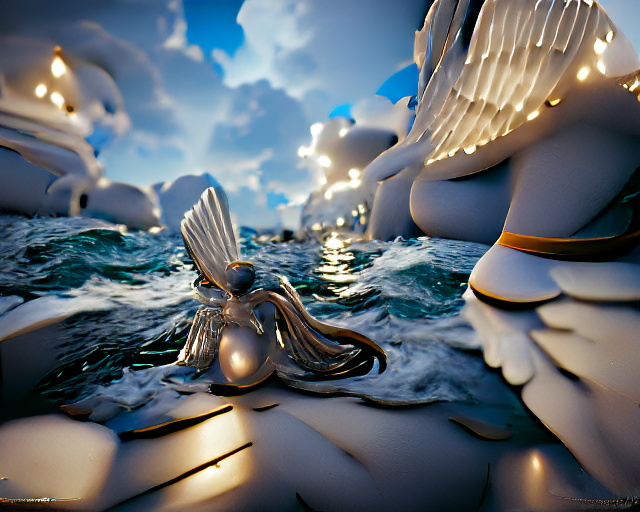
\includegraphics[width=0.7\textwidth]{img/vqgan_image.png}
    \caption{Arte generado por redes \textit{GAN} complementadas con \textit{transformers}}
    \label{fig:vqgan_image}
\end{figure}

\section{Requerimientos energéticos de las redes neuronales}
\label{sec:requerimientos_energeticos_redes_neuronales}
Las cada vez más increíbles capacidades de las redes neuronales artificiales no vienen sin coste. El coste de personal de investigación y desarrollo, así como el coste energético del proceso de entrenamiento siguen siendo exageradamente altos para proyectos complejos como los citados en la sección anterior.

Sin embargo, en este trabajo no se trata el proceso de desarrollo y entrenamiento, ya que eso se delega en los numerosos y muy competentes ingenieros en inteligencia artificial. En este trabajo se trata el proceso de inferencia, es decir, la ``ejecución'' de una red creada y entrenada.

El proceso de inferencia es mucho más sencillo y computacionalmente menos demandante que el de entrenamiento, pero tras esa falsa sensación de ``gratuidad'' de bajos recursos computacionales se oculta una trampa en la escala de dichos recursos. Esto es debido a que, a pesar de que una red neuronal durante el proceso de desarrollo se entrena múltiples veces con un elevado coste asociado, este entrenamiento habitualmente se lleva a cabo por un pequeño grupo de ingenieros. Por otro lado, si bien la ejecución de redes neuronales es mucho más barata computacionalmente hablando, la escala de estas redes neuronales, especialmente de las que aspiran a convertirse en parte de nuestras vidas, hace que un consumo de unos pocos mWh se convierta en varios kWh o incluso MWh por dispositivo a lo largo de todo el planeta.

Añadiendo a esto que se pretende que en el futuro prácticamente cualquier bien de consumo tenga inteligencia artificial asociada, la demanda de energía pasa a ser una preocupación importante, en la escala de los TWh. Es debido a esto que reducciones del consumo en pocos puntos porcentuales, a pesar de parecer logros menores, son muy importantes para la sostenibilidad a largo plazo de nuestro planeta y estilo de vida.

\section{Investigación y optimizaciones propuestas}
\label{sec:investigacion_optimizaciones_propuestas}
Como ya se comentó en la Sección \ref{sec:redes_neuronales}, la multiplicación de matrices es parte fundamental e imprescindible de la ejecución de redes neuronales no convolucionales. Esto se puede visualizar mejor en la Figura \ref{fig:profiling_several_nns}, donde se muestra en qué cargas de trabajo se invierten más ciclos en varias redes neuronales de referencia \cite[Figura 3.4]{deep_learning_for_computer_architects}. Como es de esperar, en las redes que no requieren de convolución para su funcionamiento, el porcentaje del tiempo que se dedica a la multiplicación de matrices es muy elevada, por lo que atacar dicho punto parece la decisión correcta. Sin embargo, como ingeniero informático, la optimización del algoritmo de multiplicación de matrices generales no parece un campo poco trabajado y abordable para una persona sin formación específica en matemáticas y algoritmia avanzada.

\begin{figure}[h!]
    \centering
    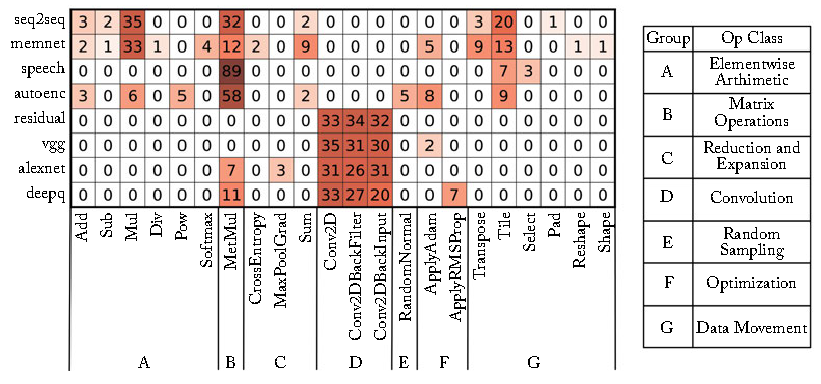
\includegraphics[width=\textwidth]{pdf_tex/dlfca_figure3_4.pdf}
    \caption{Tiempo empleado en funciones (\%) según el tipo de red neuronal}
    \label{fig:profiling_several_nns}
\end{figure}

Tras la multiplicación de matrices, las cargas de trabajo más habituales siguen estando relacionadas con el tamaño del modelo, siendo estas operaciones \textit{elementwise}, es decir, que afectan a elementos individualmente, como la multiplicación, suma o división. Por último, otra gran carga de trabajo, y gran fuente de gasto de energía, es el movimiento de datos en memoria.

Solventar estos problemas no es tarea trivial. Teniendo en cuenta la Ley de Moore, que señala cómo cada poco tiempo se dobla la cantidad de transistores en \acrshort{cpu}s, se podría pensar que esto lleva asociado un aumento en la eficiencia energética. Sin embargo, el fenómeno causante de un aumento de los FLOPs por vatio históricamente ha sido en realidad el escalado de Dennard\footnote{\url{https://en.wikipedia.org/wiki/Dennard_scaling}}, escalado que hace años que dejó de cumplirse\footnote{\url{https://cartesianproduct.wordpress.com/2013/04/15/the-end-of-dennard-scaling/}}. Conforme la industria se acerca al límite teórico del silicio, y con efectos cuánticos cada vez más presentes, una reducción o estancamiento en el tamaño de las redes no se contempla como una solución asumible. Sin embargo, que las redes no se puedan reducir en tamaño manteniendo el mismo esquema de conexiones denso, no implica que no se pueda conservar el tamaño de la red alterando el esquema de conexiones. Es aquí donde las redes neuronales dispersas comienzan a destacar como una opción con menor necesidad de FLOPs y, por tanto, con menor consumo teórico de energía, siendo particularmente útiles si se acompañan de hardware diseñado específicamente para su ejecución.

\subsection{Podado y redes dispersas}
\label{ssec:podado_y_redes_dispersas}
Mediante el proceso de podado, una red neuronal puede ver enormemente mejorado su rendimiento a costa de pequeños descensos en la precisión hasta cierto umbral. Encontrar este \textit{sweet-spot} es crucial si se desea una implementación competente, pero a la vez lo más eficiente posible. En la Figura \ref{fig:grafica_sparse_vs_dense} \cite{neuralmagic_pruning_overview} se puede apreciar cómo la precisión va progresivamente cayendo a medida que el rendimiento aumenta.

\begin{figure}[h!]
    \centering
    \vspace*{0.5cm}
    \def\svgwidth{0.9\textwidth}
    \input{pdf_tex/grafica_sparse_vs_dense/grafica_sparse_vs_dense.pdf_tex}
    \caption{Comparación de rendimiento y precisión con una red neuronal dispersa}
    \label{fig:grafica_sparse_vs_dense}
\end{figure}

Como se puede observar, en el correcto podado de redes neuronales se puede encontrar una posible solución a la elevada potencia de cómputo necesaria para la ejecución de las mismas. Sin embargo, el podado solamente ofrece resultados extraordinarios con precisiones extraordinariamente bajas, siendo deseable un equilibrio entre rendimiento y precisión. Este comportamiento no debe ser desmotivador, puesto que con las herramientas, profesionales, e investigación adecuados, estas tecnologías basadas en redes neuronales dispersas probablemente tengan un amplio margen de mejora mediante optimizaciones, arquitecturas y procesos de entrenamiento específicos.

\subsection{XPU: \textit{X Processing Unit}}
\label{ssec:xpu}
Otra posible vía de mejora de esta eficiencia es mediante la creación de circuitos de aplicación específica para inferencia, un camino muchísimo más barato de señalar que de recorrer.

Un circuito de aplicación específica o \acrshort{asic} (\textit{\acrlong{asic}}) por sus siglas en inglés es probablemente lo más alto que se puede llegar en cuanto a eficiencia de cómputo de un \textit{workload}, pero también es lo que incurre en más gastos derivados de su desarrollo. Estos costes se sitúan en los (miles de) millones de euros, y el proceso de diseño es especializado, costoso, y muy punitivo si se descubren errores graves en el diseño. Es por esto que diseñar un \acrshort{asic} para inferencia es una tarea al alcance de muy pocos.


Sin embargo, esto no ha frenado a los grandes en el universo de la \acrshort{ia} en su afán por más rendimiento y flexibilidad. Circuitos como la \acrshort{tpu} (\textit{\acrlong{tpu}}) de Google son ya una realidad. En la Figura \ref{fig:tpu_block_diagram} \cite{jouppi2017_in_datacenter_tpu} se puede ver el diagrama de bloques del chip TPU. En esta imagen se puede observar cómo un componente principal de dicho chip es el multiplicador de matrices. Este componente (entre otros) hace que esta pieza de hardware tenga un rendimiento y eficiencia muy superiores a sus contrapartes \acrshort{cpu} y \acrshort{gpu}, como se muestra en la Figura \ref{fig:tpu_benchmarks} \cite{devopedia_tpu}.

\begin{figure}[h!]
    \centering
    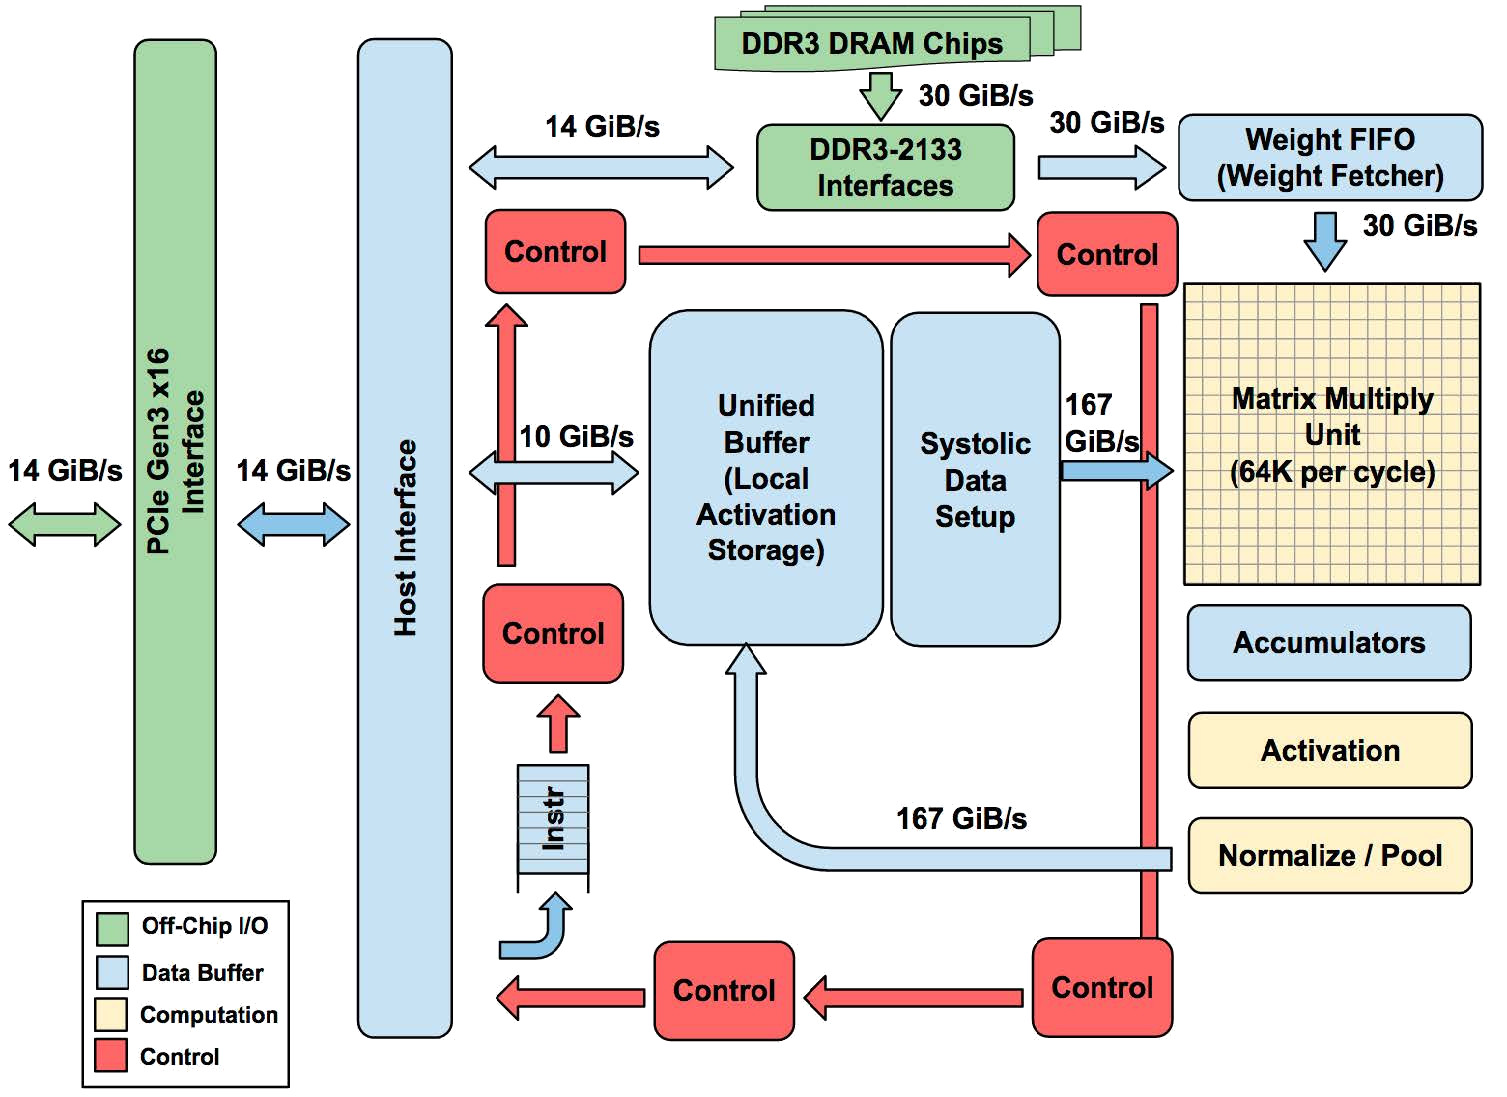
\includegraphics[width=0.85\textwidth]{img/tpu_block_diagram.jpg}
    \caption{Diagrama de bloques del chip TPU de Google}
    \label{fig:tpu_block_diagram}
\end{figure}

\begin{figure}[h!]
    \centering
    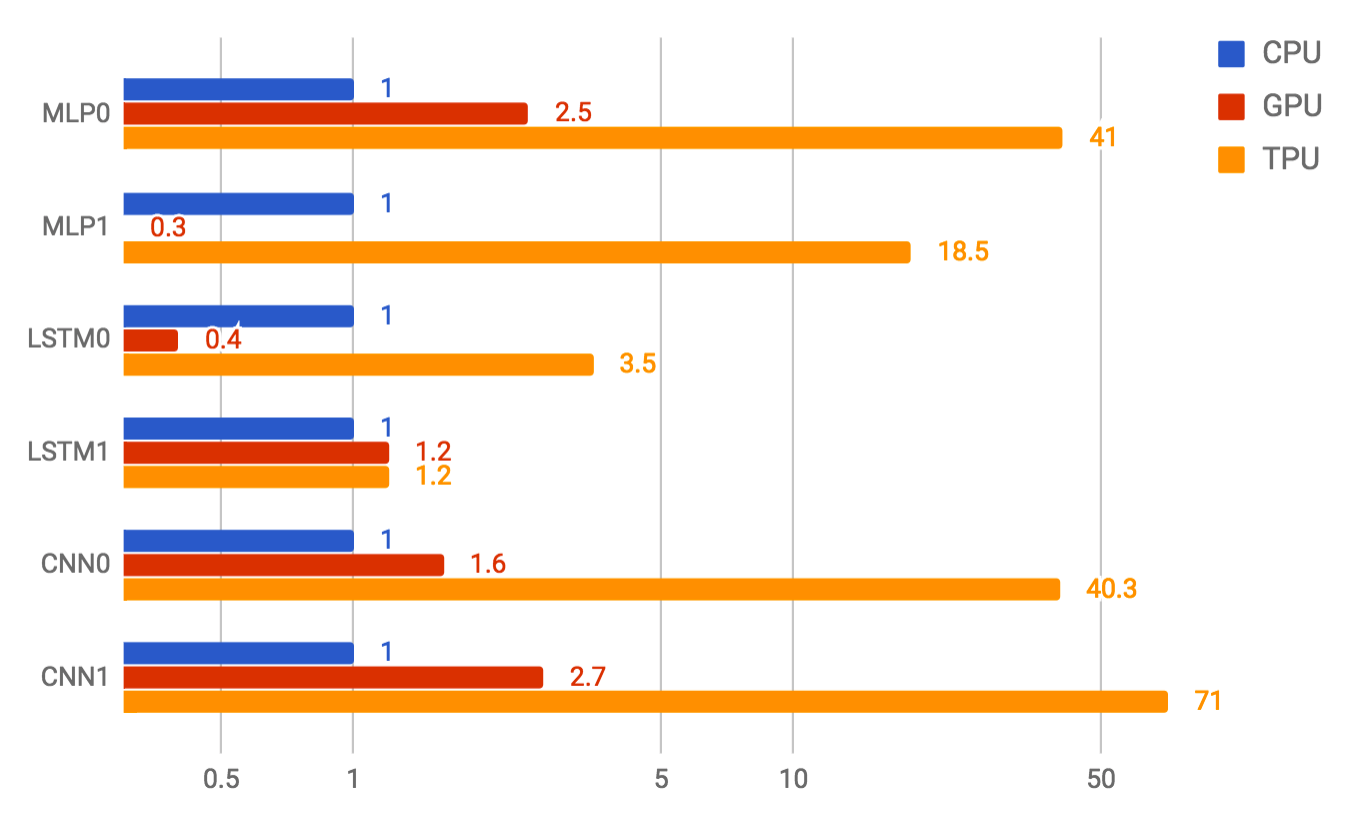
\includegraphics[width=0.85\textwidth]{img/tpu_benchmarks.png}
    \caption{Resultados del chip TPU de Google en comparación con otras alternativas}
    \label{fig:tpu_benchmarks}
\end{figure}

\subsection{Otras optimizaciones}
\label{ssec:otras_optimizaciones}
Existen también otras optimizaciones como el uso de DRAM aproximada. Estas son redes neuronales re-entrenadas sobre una plataforma con memoria de acceso aleatorio que pueda incurrir en fallos en la transferencia de datos. Dichas redes pueden aprender a identificar estos errores y adaptarse a ellos, usando tanto mecanismos explícitamente diseñados para ello como de forma automática \cite{deep_learning_for_computer_architects} \cite{koppula2019eden}. Si bien esta aproximación reduce la precisión de la red (de igual forma que lo hacen las previamente discutidas), el ahorro de energía en accesos a memoria, que supone gran parte del consumo total de energía en sistemas embebidos, puede marcar la diferencia si se encuentra el equilibrio entre precisión y consumo.
\chapter{Desarrollo y Prueba de Concepto}
\label{chap:desarrollo_poc}

\lettrine{U}{na} vez identificados los puntos de intervención y posible mejora, así como revisados los trabajos ya realizados, en este capítulo se detalle el desarrollo de una prueba de concepto.

% a pesar de que es más que probable que esta primera aproximación básica no mejore los optimizados procesos que utilizan las librerías más empleadas en este campo.

\section{Objetivos de la Prueba de Concepto}
\label{sec:objetivos_poc}
El objetivo de esta Prueba de Concepto es implementar una red neuronal para la posterior medida de su rendimiento y perfilado. Sin embargo, dado que uno de los \textit{frameworks} predominantes en la industria es \acrlong{tf}, tal como se comenta en la Sección \ref{} \textbf{TODO REF}, se han decidido desarrollar las redes neuronales mediante este \textit{framework}, ahorrando toda la implementación del entrenamiento (que no concierne a este trabajo). Esto permite no solo investigar acerca de la implementación a bajo nivel de esta librería, sino además comparar los resultados que arroja la implementación de la \acrshort{poc} con los de dicha librería, verificando así que el programa sea correcto.

Por último, el uso de \acrlong{tf} también es necesario para el podado de redes neuronales, donde es importante que la forma de las matrices sea algo extrapolable a una red neuronal real.

Para cumplir estos objetivos se crea un \textit{Jupyter Notebook} en el cual se pueden ir ejecutando paso a paso cada etapa en la generación y entrenamiento de la red, así como opcionalmente crear una variante podada del modelo, para finalmente generar código C. Los pasos para la ejecución del programa, así como los conocimientos necesarios para comprender las necesidades del mismo se describen a continuación.

A pesar de que el perfilado de un código \textit{machine learning} y extracción de sus características no precisa de ningún tipo de generación dinámica de código C, se ha decidido realizar esto y no una simple medida de rendimiento en el propio \acrlong{tf} para mejorar los conocimientos y comprensión de estas redes a bajo nivel. Esto, a pesar de que esto pueda mermar la cantidad de arquitecturas de red diferentes que se pueden medir, resulta particularmente útil a la hora de continuar la investigación realizada en redes punto a punto. 

\section{Extracción de valores para modelos TensorFlow}
\label{sec:extraccion_valores_modelo_tf}
El primer paso para la implementación de esta \acrshort{poc} es la extracción de los valores desde el modelo TensorFlow. Este modelo puede venir dado previamente en formato \texttt{.pb} (formato de archivo que emplea \acrlong{tf} en el que viene definida la arquitectura de red, así como los valores de los pesos, \textit{bias}, etc), o se puede crear y entrenar directamente desde Python sin importarlo u exportarlo en ningún momento.

Como los modelos más grandes y complejos no suelen ser modelos exclusivamente \textit{feed-forward} con funciones de activación exclusivamente sigmoides (\textbf{TODO REF SECCION 2}), lo más cómodo es simplemente generar una red neuronal de pruebas, entrenarla, y exportar el resultado a C.

\subsection{Desde un modelo guardado}
\label{ssec:desde_modelo_guardado}
Para realizar esto, que queda fuera del objetivo de este trabajo, bastaría con emplear la función \texttt{saved\_model.load} de TensorFlow sobre un modelo \texttt{.pb} previamente exportado \cite{tensorflow_saved_model}. Esto permitiría importar grandes modelos preentrenados y realizar mediciones sobre modelos ``del mundo real'', pero implicaría una gran cantidad de horas de trabajo y adaptación, debido a la gran cantidad de parámetros, tipos de capas y funciones de activación, entre otros, que no se han implementado.

Por esta razón, este proyecto se limita a la extracción para modelos puramente \textit{feed-forward} con función de activación sigmoide (a pesar de que añadir soporte para distintas funciones de activación sería relativamente sencillo de implementar).

\subsection{Desde un modelo de pruebas}
\label{ssec:desde_modelo_de_pruebas}
Este es el camino más sencillo a la hora de implementar lo que, recordemos, es simplemente un laboratorio básico para poder realizar mediciones y extraer conclusiones.

\subsubsection{Fase común}
\label{sssec:modelo_pruebas_fase_comun}
A continuación se muestran, por orden de aparición en el \textit{notebook}, los pasos de entrenamiento de la red.

\begin{enumerate}
    \item Se importa el conjunto de datos. En este caso se ha empleado el \textit{dataset} \texttt{german\_credit\_numeric}, debido a la simplicidad de sus entradas y salidas, así como por los numerosos ejemplos disponibles para este. Este conjunto de datos cuenta con 1000 datos de entrada de 24 parámetros numéricos cada uno, y se emplea para intentar parametrizar el riesgo crediticio de un individuo mediante redes neuronales.\medskip
\begin{lstlisting}[language=Python]
ds = tfds.load('german_credit_numeric', split='train', as_supervised=True)
\end{lstlisting}

    \item Se indican la función de pérdida, el optimizador y la métrica. Esto, si bien sería un tema muy interesante si este trabajo tratase de obtener buenos resultados con esta red, en este caso es irrelevante que la arquitectura de la red sea buena o no, así como la calidad de su entrenamiento y resultados.

    \item Se crea un modelo secuencial, es decir, un modelo ``capa por capa'', en el que cada capa va a continuación de la siguiente. Tras crearlo se \textit{buildea} (\texttt{model.build()}) y se compila.\medskip
\begin{lstlisting}[language=Python]
model = tf.keras.models.Sequential(name= "MySampleModel")
model.add(tf.keras.layers.InputLayer((tamano_entrada,)))
model.add(tf.keras.layers.Dense(units = h0_size, activation="sigmoid"))
model.add(tf.keras.layers.Dense(units = h1_size, activation="sigmoid"))
model.add(tf.keras.layers.Dense(units = 1, activation="sigmoid"))

model.build()

model.compile(loss=fn_perdida, optimizer=optimizador, metrics=metrica)
\end{lstlisting}

    \item Tras la creación del modelo hay que entrenarlo. Este complejo proceso a nivel de implementación, basado en el algoritmo de \textit{backpropagation}, y con todos los detalles que este implica, se puede realizar en, al más puro estilo Python, con un \textit{one-liner}.\medskip
\begin{lstlisting}[language=Python]
history =  model.fit(x=lote_entrenamiento[0], y = lote_entrenamiento[1], batch_size = 20, epochs=num_epochs)
\end{lstlisting}
\end{enumerate}

\subsubsection{Fase de podado}
\label{sssec:modelo_pruebas_fase_podado}
En caso de querer podar la red para aumentar su \textit{sparsity}, el procedimiento es muy similar al descrito en \cite{tensorflow_prune_model}. Los pasos para realizar este procedimiento se describen a continuación:
\begin{enumerate}
    \item Se crean los parámetros para podar el modelo hasta una \textit{sparsity} en este caso del 80\%. Previo al podado se copia el modelo original a un modelo diferente, \texttt{model\_for\_pruning}.\medskip
\begin{lstlisting}[language=Python]
prune_low_magnitude = tfmot.sparsity.keras.prune_low_magnitude

batch_size = 20
sparse_epochs = 2
validation_split = 0.1

end_step = np.ceil(tamano_lote/batch_size).astype(np.int32) * sparse_epochs

pruning_params = {
    'pruning_schedule': tfmot.sparsity.keras.PolynomialDecay(
        initial_sparsity=0,                                                    
        final_sparsity=0.8,
        begin_step=0,
        end_step=end_step
    )
}

# clone the model. If we do not do this, the original model will be altered too
model_for_pruning = tf.keras.models.clone_model(model)

model_for_pruning = prune_low_magnitude(model_for_pruning, **pruning_params)

# `prune_low_magnitude` requires a recompile.
model_for_pruning.compile(optimizer=optimizador, # 'adam',
                loss=fn_perdida,
                metrics=metrica)

model_for_pruning.summary()
\end{lstlisting}
    \item Se entrena el modelo podado. Este procedimiento es muy similar al entrenamiento en una línea explicado previamente, únicamente añadiendo el \textit{callback} necesario para el entrenamiento de un modelo podado.
\begin{lstlisting}[language=Python]
num_epochs =  500

callbacks = [
    tfmot.sparsity.keras.UpdatePruningStep(),
]

history = model_for_pruning.fit(lote_entrenamiento[0], lote_entrenamiento[1], batch_size=batch_size, epochs=num_epochs, validation_split=validation_split, callbacks=callbacks)
history.history
\end{lstlisting}
\end{enumerate}

\subsection{Extracción de valores}
\label{ssec:extraccion_valores}
Ahora que se cuenta con un modelo de red neuronal de discutible calidad, pero funcionalmente idéntico a otro mejor adaptado al problema a resolver, se puede comenzar con la extracción de valores de cada capa.

\begin{enumerate}
    \item Primero es necesario obtener tanto los pesos como los \textit{bias}. Para esto se itera sobre las capas del modelo. En cada capa del modelo se puede llamar a la función \texttt{get\_weights()}. En el resultado que devuelve, los pesos se encuentran en un array de arrays en la posición 0, y los \textit{bias} un array en la posición 1.\medskip
\begin{lstlisting}[language=Python]
for layer in model.layers:
    print(f"LAYER{idx}_WEIGHTS:")
    print(layer.get_weights()[0])
    print(f"LAYER{idx}_BIAS:")
    print([layer.get_weights()[1]])

# LAYER1_WEIGHTS:
# [[-0.08928536  0.08118167 -1.6078503  -0.29092655 -0.33163825]
#                               ...
#  [-0.16627118 -0.36254594  0.03569769  0.11377215 -0.19968267]]
# LAYER1_BIAS:
# [ 0.00605693  0.00038876  0.29822487  0.01296887 -0.02708104]
# LAYER2_WEIGHTS:
# [[-0.43815556  0.6910728   0.45901924]
#                   ...
#  [ 1.3233485  -0.26594874 -0.5277702 ]]
# LAYER2_BIAS:
# [-0.1541544  -0.04604432  0.15921216]
# LAYER3_WEIGHTS:
# [[-3.4663067 ]
#       ...
#  [ 1.5324626 ]]
# LAYER3_BIAS:
# [1.3300072]
\end{lstlisting}
    Sin embargo, esta aproximación es problemática a la hora de obtener los pesos. Y es que al mostrar los pesos en formato humano (decimal), se pierde precisión. Para solucionar esto se necesita algo más directo y de bajo nivel.
    
    \item La solución a la que se ha llegado es la más evidente, exportar los datos en formato máquina, es decir, binario codificado en hexadecimal. Realizar esto en Python no es particularmente difícil, y si bien existen mejores formas de interfacear con código C, se ha de recordar que esto es simplemente una prueba de laboratorio y no un producto final. De esta forma, se define una función para la conversión de datos en hexadecimal:\medskip
\begin{lstlisting}[language=Python]
# https://docs.python.org/3/library/struct.html
FLOAT_BE = ">f"
FLOAT_LE = "<f"
DOUBLE_BE = ">d"
DOUBLE_LE = "<d"

def np_value_to_hex(value, byte_format):
    return bytearray(struct.pack(byte_format, value)).hex()

# byte_format is target format for output
def np_array_to_hex(array, byte_format):
    return map(
        lambda layer: list(
            map(lambda v: np_value_to_hex(v, byte_format), layer)
        ),
        array,
    )
\end{lstlisting}
    Y tras crear dicha función, ahora con un poco de manejo de strings, fácilmente se puede obtener un resultado como el siguiente:\medskip
\begin{lstlisting}[language=Python]
# LAYER1_WEIGHTS:
# bdb6db3e,3da64293,bfcdce0a,be94f453,bea9cc7d
#                     ...
# be2a42fe,beb99f9f,3d1237be,3de90160,be4c799d
# LAYER1_BIAS:
# 3bc67940,39cbd218,3e98b0ee,3c547b67,bcddd911
# LAYER2_WEIGHTS:
# bee055ed,3f30ea26,3eeb0492
#            ...
# 3fa9637c,be882a6f,bf071bf3
# LAYER2_BIAS:
# be1ddaa7,bd3c98f7,3e230883
# LAYER3_WEIGHTS:
# c05dd7f8
#   ...
# 3fc427bc
# LAYER3_BIAS:
# 3faa3dad
\end{lstlisting}

    \item Por último, pero no por ello menos importante, se han de exportar también los datos de entrada del propio dataset. Como se discutirá más adelante, el formato del documento que lee el código C compilado contará con una primera línea especificando el número de líneas que va a leer, y un dato por línea. De esta forma, si la entrada contiene inferir 1000 datos, el contenido del documento será de 1001 líneas, siendo la primera \texttt{1000}, y el resto conteniendo los datos a inferir.\medskip
\begin{lstlisting}[language=Python]
# Get original stdout here, in order to print to a file
my_stdout = sys.stdout

with open('input.txt', 'w') as f:
    sys.stdout = f
    # Print dims to beginning of file
    print(len(lote_entrenamiento[0]))
    # and data to the rest of it
    for arr in lote_entrenamiento[0]:
        print(*arr.numpy().tolist(), sep=',')
    # Finally restore stdout
    sys.stdout = my_stdout
\end{lstlisting}
    Al ejecutar el código anterior, se crea en el directorio de trabajo el fichero \texttt{input.txt}, que contiene un total de 1000 entradas en este caso. Para este ejemplo, el fichero se ha recortado a 5 entradas por conveniencia.\medskip
\begin{lstlisting}
5
3,6,4,13,2,5,1,4,3,28,3,2,2,2,1,1,0,1,0,0,1,0,0,1
4,4,2,6,1,2,2,3,1,23,3,1,2,1,1,0,0,1,0,1,0,0,1,0
4,24,4,20,1,3,2,4,3,37,3,1,1,2,1,1,0,1,0,0,1,0,0,1
4,18,2,11,5,2,2,2,1,21,3,1,1,2,1,0,0,1,0,1,0,0,0,1
4,6,2,13,3,3,1,4,1,62,3,1,1,1,1,0,0,1,0,0,1,0,0,1
\end{lstlisting}

    Conviene recalcar que en este caso el tipo de los datos de entrada es entero. En caso de ser datos en coma flotante, se procedería, en función de la relevancia de la precisión de los datos, a exportar en formato decimal (precisión poco relevante) o hexadecimal (precisión muy relevante).
\end{enumerate}

\subsubsection{Extracción de datos dispersos}
\label{sssec:extraccion_datos_dispersos}
Para la extracción de datos dispersos se procede de igual forma que con datos densos. Iterando a través de cada una de las capas con funciones como las expuestas previamente, se obtienen resultados como el siguiente:\medskip
\begin{lstlisting}[language=Python]
# LAYER1_WEIGHTS:
# 80000000,80000000,00000000,00000000,00000000
#                     ...
# 3ec9393d,80000000,80000000,00000000,00000000
# LAYER1_BIAS:
# 39fcfbe4,3854f5e8,b82401d6,b8b52b95,ba28adf7
# LAYER2_WEIGHTS:
# 80000000,00000000,80000000
#            ...
# 80000000,80000000,3f5a98cf
# LAYER2_BIAS:
# 3bea3c98,3d964016,3b89974c
# LAYER3_WEIGHTS:
# 80000000
#   ...
# 3f61fe09
# LAYER3_BIAS:
# 3ec81415    
\end{lstlisting}

Como se puede apreciar dentro de las zonas recortadas, la mayor parte de datos son 0x80000000 o 0x00000000, siendo ambos representaciones del número cero en coma flotante. Con ayuda de la función \texttt{nonzero} de \texttt{numpy} se puede extraer fácilmente cada valor diferente de cero con sus coordenadas verticales y horizontales para importar más adelante en C, tal como se muestra en la siguiente sección.

\section{Importación de valores en C}
\label{sec:importacion_valores_c}
En esta sección se describe cómo se importan los datos extraídos de los modelos \acrshort{tf} densos o dispersos, creados en la sección anterior.

\subsection{Importación de matrices densas}
\label{ssec:importacion_matrices_densas}
El lenguaje de programación C almacena las matrices por filas. Aprovechando esta característica, y haciendo uso del tan granular acceso a bajo nivel que nos permite hacer este lenguaje, se importan las matrices de pesos y \textit{bias} de las diferentes capas desde la zona de memoria constante, o para x86, la sección \texttt{.text}. Esto implica que, una vez que el programa se carga en memoria, este no lee ningún archivo salvo la entrada de datos.

Mediante funciones de manejo de \textit{strings} en Python para la generación de estas líneas de código, y recordando que la arquitectura x86(y \_64) es \textit{little endian}\footnote{\url{https://es.wikipedia.org/wiki/Endianness}}, los valores constantes se importan al código con las siguientes líneas:\medskip
\begin{lstlisting}[language=C]
#define INPUT_SIZE 24
#define LAYER1_SIZE 5
const fp32 * layer1_weights = (fp32 *)
        "\xf3\x79\x85 /* [...] */ \x8c\xab\xbe";
const fp32 * layer1_bias = (fp32 *)
        "\x3f\x1b\x5f /* [...] */ \x54\x37\x3c";
#define LAYER2_SIZE 3
const fp32 * layer2_weights = (fp32 *)
        "\x16\xbd\xc5 /* [...] */ \x8d\x77\x3f";
const fp32 * layer2_bias = (fp32 *)
        "\xfc\x06\x25 /* [...] */ \xa4\x2a\xbe";
#define LAYER3_SIZE 1
const fp32 * layer3_weights = (fp32 *)
        "\x09\x88\x1d /* [...] */ \x57\x04\x40";
const fp32 * layer3_bias = (fp32 *) "\xc8\x2d\x40\x3d";
\end{lstlisting}

Estos valores, al ser \textit{casteados} a un vector de \texttt{fp32}, pueden ser accedidos más adelante con el \textit{stride} de dicho tipo de dato (en este caso, 32 bits).

\subsection{Importación de matrices dispersas}
\label{ssec:importacion_matrices_dispersas}
En el caso de las matrices dispersas el almacenamiento de datos no es tan sencillo. Como se comenta en el Capítulo \ref{chap:conceptos_basicos}, existen múltiples formatos de representación de matrices dispersas en memoria. El formato que se emplea en la creación de dicha matriz es la \acrshort{coo} (Subsección \ref{ssec:almacenamiento_matrices_dispersas}). De esta manera, es suficiente con exportar una lista de valores acompañado con las coordenadas de cada uno de ellos. Estos valores, tanto los de la matriz como las coordenadas de los mismos, y de igual manera que en la Subsección \ref{ssec:importacion_matrices_densas}, se guardan en la sección de texto.

Esto significa que, en comparación con la versión densa, el vector de pesos es mucho más pequeño (en función de la densidad de la matriz que representa), y aparecen dos vectores de coordenadas, que identifican las abscisas y ordenadas de cada dato \textit{nonzero}, siendo estos \texttt{i} y \texttt{j}, respectivamente:\medskip
\begin{lstlisting}[language=C]
#define INPUT_SIZE 24
#define LAYER1_SIZE 5
#define layer1_nz 24
const fp32 * layer1_weights = (fp32 *)
        "\x7c\xce\xbc /* [...] */ \x39\xc9\x3e";
const int layer1_i[layer1_nz] =
        {1,1,2,3,3,4,8,11,12,12,13,14,15,15,15,17,18,18,19,19,20,21,21,23};
const int layer1_j[layer1_nz] =
        {0,1,1,1,2,0,3,2,1,2,1,4,1,2,4,3,1,2,0,1,2,3,4,0};
const fp32 * layer1_bias = (fp32 *)
        "\xe4\xfb\xfc /* [...] */ \xad\x28\xba";
#define LAYER2_SIZE 3
#define layer2_nz 3
const fp32 * layer2_weights = (fp32 *)
        "\xe2\x81\x50 /* [...] */ \x98\x5a\x3f";
const int layer2_i[layer2_nz] = {2,3,3};
const int layer2_j[layer2_nz] = {2,0,2};
const fp32 * layer2_bias = (fp32 *)
        "\x98\x3c\xea /* [...] */ \x97\x89\x3b";
#define LAYER3_SIZE 1
#define layer3_nz 1
const fp32 * layer3_weights = (fp32 *) "\x09\xfe\x61\x3f";
const int layer3_i[layer3_nz] = {1};
const int layer3_j[layer3_nz] = {0};
const fp32 * layer3_bias = (fp32 *) "\x15\x14\xc8\x3e";
\end{lstlisting}


\section{Generación dinámica de código C a partir del modelo TensorFlow}
\label{sec:generacion_din_modelo_tf}
Tras ver cómo extraer los valores de pesos, \textit{bias} y datos de entrada del entorno de \acrlong{tf}, se cuenta con todas las herramientas necesarias para generar el código C, o código para prácticamente cualquier lenguaje si se cuenta con los conocimientos adecuados.

\subsection{Decisiones previas de diseño}
\label{ssec:decisiones_previas_diseno}
Las funciones, definiciones de tipo, y otros recursos comunes a todos los códigos generados, sean estos densos o dispersos, se han centralizado en los ficheros \texttt{common.\{c|h\}}. Primeramente, se ha decidido emplear un tipo \texttt{union} para la implementación de los datos en coma flotante, al permitir estos un control superior a nivel de byte, sin complicaciones adicionales como \textit{casting} de punteros. Los únicos dos tipos de datos implementados son \texttt{fp32} y \texttt{fp64}, con nombres representativos de su precisión. Por ejemplo, el tipo \texttt{union} para el flotante de 32 bits es el siguiente:\medskip
\begin{lstlisting}[language=C]
typedef union _fp32 {
    uint32_t raw;
    float val;
    uint8_t byte[4];
} fp32;
\end{lstlisting}

Así, las funciones implementadas tendrán versiones para flotantes de 32 y 64 bits. El sufijo que indica la precisión del flotante será \texttt{\_\_fp32} y \texttt{\_\_fp64} para 32 y 64 bits de precisión, respectivamente. Las pocas funciones implementadas han sido necesarias para la aplicación del \textit{bias}, y siguen esta nomenclatura con el propósito de mejorar una futura parametrización extra en la generación de código.

Se ha barajado también la posibilidad de emplear funciones genéricas que brinda el compilador gcc, pero al final por simplicidad, y dada la naturaleza estática de una Prueba de Concepto, se ha optado por no incluir estas macros. Un ejemplo para la función \texttt{fast\_sigmoid} sería el siguiente:\medskip
\begin{lstlisting}[language=C]
#define fast_sigmoid(X) _Generic((X), \
fp32:fast_sigmoid__fp32, \
fp64:fast_sigmoid__fp64 \
)(X)

#pragma inline fast_sigmoid__fp32, fast_sigmoid__fp64
fp32 fast_sigmoid__fp32(fp32);
fp64 fast_sigmoid__fp64(fp64);
\end{lstlisting}


\subsection{Matrices densas}
\label{ssec_gdin_matrices_densas}
La forma más sencilla (y cronológicamente la primera en ser implementada) es la basada en matrices densas. Esta implementación se apoya en la ampliamente disponible librería \texttt{OpenBLAS}\footnote{\url{https://www.openblas.net}}. A pesar de que el proceso de desarrollo, pruebas, automatización y corrección de posibles bugs pueda ser algo tedioso, en realidad la teoría es moderadamente simple.

Tal como se comenta en la Sección \ref{sec:redes_reuronales_densas}, el programa debe hacer lo siguiente:

\begin{enumerate}
    \item Leer los datos de entrada.
    \item Multiplicar los datos de entrada por cada una de las capas.
    \item Tratar adecuadamente los datos de salida.
\end{enumerate}

Estos tres sencillos pasos tienen su complicación, debido a que hay que implementar todo desde cero y automatizar su generación. Para cada punto anterior, la estructura básica del programa debe ser la siguiente:

\begin{enumerate}
    \item Leer los datos de entrada es quizás de lo más sencillo. Es manejo de ficheros básico mediante \texttt{fscanf}:\medskip
\begin{lstlisting}[language=C]
FILE *inputfile;
fprintf(stderr, "*** Opening %s as input ***\n", argv[1]);
if((inputfile = fopen(argv[1], "r")) == NULL){
    fprintf(stderr, "  -> Error: file %s does not exist\n", argv[1]);
    exit(-1);
}

// Parse input dims and allocate memory consequently
int input_dim;
fscanf(inputfile, "%d", &input_dim);

fp32 * input;
input = malloc(input_dim * INPUT_SIZE * sizeof(fp32));

// Read input
for(int i = 0; i < INPUT_SIZE * input_dim; i++){
    fscanf(inputfile, "%f,", &input[i].val);
}

// Finish reading input so let's close it
fclose(inputfile);
\end{lstlisting}

    \item Para realizar la multiplicación de matrices, y siguiendo con este ejemplo, se emplea la función \texttt{cblas\_sgemm}. Esta función realiza un producto de matrices ampliado tal que $C = \alpha AB + \beta C$. El resultado se guarda de forma aditiva sobre $C$, por lo que es necesario que o bien dicha matriz esté a cero, o el factor $\beta$ sea cero.\medskip
\begin{lstlisting}[language=C]
fprintf(stderr, "*** SGEMM %s x %s ***\n", "layer0", "layer1");
cblas_sgemm(CblasRowMajor, CblasNoTrans, CblasNoTrans, input_dim,
            LAYER1_SIZE, LAYER0_SIZE, 1.f, (float *) layer0_out,
            LAYER0_SIZE, (float *) layer1_weights, LAYER1_SIZE,
            0.f, (float *) layer1_out, LAYER1_SIZE);
\end{lstlisting}

    Tras la multiplicación de $A$ por $B$, aditiva sobre $C$, se han de aplicar los \textit{bias} y la función de transferencia. Esto se realia con una función ad-hoc que combina ambas acciones en un solo recorrido lineal por memoria: \texttt{map\_and\_bias}.
\begin{lstlisting}[language=C]
fprintf(stderr, "*** Map and Bias %s with %s function ***\n", "layer1_out", "sigmoid__fp32");
map_and_bias__fp32(layer1_out, layer1_bias, input_dim, LAYER1_SIZE, 'N', sigmoid__fp32);
\end{lstlisting}

    Si bien es cierto que en lugar de aplicar los \textit{bias} junto a la función de transferencia en la función previa, es posible realizar $C = AB + bias$, con una copia de \textit{bias} por fila, es mejor realizar esta operación en conjunción con la aplicación de la función de transferencia, ya que así se obtiene una mayor intensidad aritmética. Esta mayor intensidad aritmética es especialmente relevante cuando una función se paraleliza, ya que lo más probable es que \texttt{map\_and\_bias} sea \textit{memory-bound} en mayor o menor medida en función de la función de transferencia. Además, si se realizara operación sobre una matriz pre-inicializada con los \textit{bias} en cada fila, se necesitaría replicar los valores de \textit{bias} \texttt{input\_dim}\footnote{Se denomina \texttt{input\_dim} al número de filas de la entrada, es decir, el número de datos multidimensionales que entran a la red.} veces, replicación que no es gratuita.

    Una implementación básica de \texttt{map\_and\_bias} es similar a la siguiente:
\begin{lstlisting}[language=C]
void map_and_bias__fp32(fp32 *restrict A, const fp32 *restrict bias, const uint32_t M, const uint32_t N, fp32 (* map_function)(fp32 x)){
    for (uint32_t i = 0; i < M; i++){
        for(uint32_t j = 0; j < N; j++){
            A[i*N+j].val = map_function((fp32)(A[i*N+j].val +
                                        bias[j].val)).val;
        }
    }
}
\end{lstlisting}

    \item Tras repetir el paso anterior tantas veces como capas tenga la arquitectura, la salida de cada capa \texttt{M} de la red se puede encontrar en \texttt{layerM\_out}, pudiéndose encontrar la salida de la red en la matriz \texttt{layerN\_out} para una red de \texttt{N} capas. Estos datos pueden ser exportados, mostrados, contados, posprocesados, etc. Como en este caso interesa perfilar y visualizar las características del \texttt{workload}, lo más lógico es primero probar con una cantidad reducida de datos para verificar el correcto funcionamiento del código generado.
    
    Tras verificar el correcto funcionamiento de la red, y observar que para las implementaciones con \texttt{OpenBLAS} y \texttt{librsb}, los resultados son exactamente iguales a los proporcionados por \texttt{numpy}, se añade un pequeño resumen de ejecución, que clasifica el número de predicciones mayores o menores a 0,5. Esto es realmente útil para comparar la validez de los resultados con respecto a \acrlong{tf} de forma rápida.

\begin{lstlisting}[language=C]
printf("\n\n--- SUMMARY ---\n");
printf(" - Batch size = %d\n", input_dim);
printf(" - Total >0.5 predictions = %d\n", greater_count);
printf(" - %% >0.5 = %.2lf%%\n", ((double) greater_count / (double) input_dim)*100);
printf("\n");
\end{lstlisting}

\end{enumerate}


\subsection{Matrices dispersas}
\label{ssec_gdin_matrices_dispersas}
Una vez detallado cómo se procede con matrices de pesos densas, y según lo visto en la Sección \ref{sec:redes_reuronales_dispersas}, los pasos a mayores que se deben realizar para implementar una red neuronal basada en matrices dispersas son:

\begin{enumerate}
    \item Transponer la entrada y salida.
    \item Ajustar los parámetros de las funciones densas.
    \item Sustituir las matrices de pesos densas por disperspasp.
    \item Sustituir las funciones densas por sus equivalentes dispersas.
\end{enumerate}

Para realizar estos pasos primero se necesita una librería \acrshort{blas} que soporte matrices dispersas y que exponga una cabecera para C. A ser posible, y como en cualquier proyecto, es conveniente que una dependencia \textit{core}, como lo es la librería de multiplicación de matrices en este caso, sea moderadamente conocida, dado que ello asegurará una mayor calidad del código interno, así como un mejor soporte. Cumpliendo estos requerimientos, se ha optado por la utilización de la librería \texttt{librsb}\footnote{Página principal \url{http://librsb.sourceforge.net}, con paquete en el AUR (ArchLinux User Repository) \url{https://aur.archlinux.org/packages/librsb}, así como parquete mantenido en Ubuntu \url{https://packages.ubuntu.com/jammy/librsb-dev}}, de la cual se emplea su interfaz \textit{Sparse BLAS}. De esta forma, los pasos para adaptar el código para trabajar con matrices de pesos dispersos son:

\begin{enumerate}
    \item Para transponer las matrices de entrada y de salida se emplea una función \textit{built-in} de OpenBLAS, por lo que en este aspecto el código está ligado a dicha librería. De todos modos, no parece una dependencia muy complicada de sobrellevar, puesto que esta implementación es muy habitual en la industria, y aún por encima es una función que solo se usará en esta prueba de concepto. A continuación se muestra cómo transponer la entrada. Para transponer la salida se procede de forma análoga, como se muestra más adelante.\medskip
\begin{lstlisting}[language=C]
fprintf(stderr, "*** Transposing input out-of-place ***\n");
cblas_somatcopy(CblasRowMajor, CblasTrans, input_dim, LAYER0_SIZE, 1.f, (float *) input, LAYER0_SIZE, (float *) temp_input, input_dim);
\end{lstlisting}

    Este procedimiento, que se realiza \textit{out-of-place} por la mejora en rendimiento que supone al transponer matrices no cuadradas, es complementado con lógica básica de punteros previa y posterior en la que no es necesario profundizar, pero que hace que esta transposición sea transparente al resto del código. A continuación se muestra como ejemplo el bloque que realiza la transposición de la capa de salida de forma transparente al resto del programa, para una red neuronal de tres capas:\medskip
\begin{lstlisting}[language=C]
#if LAYER3_SIZE != 1
fp32 * temp_output = malloc(input_dim * LAYER3_SIZE * sizeof(fp32));
fprintf(stderr, "*** Transposing output out-of-place ***\n");
cblas_somatcopy(CblasRowMajor, CblasTrans, LAYER3_SIZE, input_dim, 1.f, (float *) layer3_out, input_dim, (float *) temp_output, LAYER3_SIZE);
free(layer3_out);
layer3_out = temp_output;
temp_output = NULL;
#endif
\end{lstlisting}

    \item En cuanto a ``ajustar los parámetros de las funciones densas'', este es un paso intermedio que no se aprecia en la versión final. En este paso se comprueba que el resultado no varía al adaptar el código a las funciones \textit{sparse BLAS} de \texttt{librsb}. Fuera de los cambios en los parámetros, también se hace necesario un cambio en la función \texttt{map\_and\_bias}, que ahora debe aplicar los \textit{bias} en un \textit{layout} de memoria diferente. Para esto se añade un parámetro \texttt{transA}. Este parámetro no transpone la matriz, como si que ocurre en \textit{BLAS}, sino que más bien indica a \texttt{map\_and\_bias} que la matriz sobre la que aplica los \textit{bias} y función de transferencia está transpuesta en memoria, por lo que el \textit{traversing} debe ser diferente. La modificación de dicha función consiste en:\medskip
\begin{lstlisting}[language=C]
void map_and_bias__fp32(fp32 *restrict A, const fp32 *restrict bias, const uint32_t M, const uint32_t N, const char transA, fp32 (* map_function)(fp32 x)){
    switch (transA){
    case 'N':
    case 'n':
        // [...] algoritmo inicial
        break;

    case 'T':
    case 't':
        for (uint32_t i = 0; i < M; i++){
            for(uint32_t j = 0; j < N; j++){
                A[i*N+j].val = map_function((fp32)(A[i*N+j].val 
                                            + bias[i].val)).val;
            }                                 // ^^^^^
        }                    // aquí se cambia el orden de acceso a bias
        break;
    }
}
\end{lstlisting}

    \item El siguiente paso es sustituir las matrices de pesos densas por matrices de pesos dispersas. Para esto se emplea el mismo método de \textit{hardcodeo} de datos en la Subsección \ref{ssec:importacion_matrices_dispersas} mediante el uso de \texttt{\#define}. De esta forma, lo que previamente sería \texttt{layerN\_weights}, y una \textit{string} de datos binaros a continuación, se divide ahora en \texttt{layerN\_sp\_weights} (\textit{layerN sparse weights}, que contiene los valores distintos de cero para la matriz de pesos dispersa), así como en dos vectores de coordenadas \texttt{layerN\_i} y \texttt{layerN\_j}.
    
    Estos datos son necesarios para la creación de las matrices dispersas, indicando \texttt{layerN\_i} y \texttt{layerN\_j} la fila y la columna de cada valor en el array de pesos, respectivamente. Además, también es necesario el número de \textit{nonzeros} (\texttt{layerN\_nz}) para la creaación de dichas matrices. Sabiendo esto, las matrices dispersas se crean de la siguiente manera:
\begin{lstlisting}[language=C]
blas_sparse_matrix layer1_sp_weights = blas_invalid_handle;
/* [...] */

layer1_sp_weights = BLAS_suscr_begin(LAYER0_SIZE, LAYER1_SIZE);
BLAS_suscr_insert_entries(layer1_sp_weights, layer1_nz, (float *)
                          layer1_weights, layer1_i, layer1_j);
BLAS_suscr_end(layer1_sp_weights);
\end{lstlisting}

    \item Finalmente, queda emplear las funciones adecuadas para la mutiplicación de matrices $d\times D$. Este proceso consiste básicamente en sustituir la función \texttt{[sdcz]gemm} por una función \texttt{[sdcz]usmm} (Subsección \ref{ssec:propiedades_producto_matrices_dispersas}), así como indicar a \texttt{map\_and\_bias} que la matriz de resultados se encuentra transpuesta. Los valores de $M$ y $N$ de la matriz original no transpuesta \texttt{C}, también deben intercambiarse.
\begin{lstlisting}[language=C]
fprintf(stderr, "*** SUSMM %s(T) x %s(T) ***\n", "layer3", "layer2");
BLAS_susmm(blas_rowmajor, blas_trans, input_dim, 1.f, layer3_sp_weights,
           (float *) layer2_out, input_dim, (float *) layer3_out,
           input_dim);
fprintf(stderr, "*** Map and Bias %s(T) with %s function ***\n",
                "layer3_out", "sigmoid__fp32");
map_and_bias__fp32(layer3_out, layer3_bias, LAYER3_SIZE, input_dim,
                   'T', sigmoid__fp32);
\end{lstlisting}
\end{enumerate}

\section{Posibilidades de la generación de código}
\label{sec:posibilidades_de_la_generacion_de_codigo}
Las posibilidades de esta aproximación al análisis y medida del rendimiento son muchas. Generar código C a partir de un modelo que precisa de soporte en Python es algo especialmente útil para sistemas sin dicho soporte. Es cierto que existe TensorFlow Lite para sistemas embebidos, pero la flexibilidad que aporta crear un código C y la posibilidad de paralelizar tanto en memoria compartida como distribuida dicho código son motivos de peso.

En conjunción con todo esto, el hecho de emplear matrices dispersas viene no solamente condicionado por la literatura ya existente, que destaca los beneficios en cuanto a la proporción rendimiento/precisión de redes podadas, sino que viene también motivada por las labores de investigación en cuanto a análisis estático de código y empaquetamiento de operandos para vectorización conducidas en \cite{custom_high_performance_vector_codegen_sparse_computations}.

A continuación, se mencionan algunas de las posibilidades que abre esta posibilidad de generar código a partir de un modelo pre-entrenado.

\subsection{En plataformas de cómputo generalistas}
\label{ssec:posibilidades_en_computo_generalistas}
En el mundo de la inteligencia artificial, tanto el entrenamiento como la inferencia de redes neuronales están dominados por las \acrshort{gpu}s (\textit{\acrlong{gpu}s}). Estos dispositivos son muy convenientes para las cargas de trabajo que se manejan en deep learning, y aportan aceleraciones muy significativas sobre su contraparte en CPU. Sin embargo, los principales fabricantes de CPUs están realizando fuertes inversiones en la adaptación de sus arquitecturas tradicionales para la aceleración de \textit{workloads} de \acrshort{ia}. Fabricantes como Intel y AMD, pero también algunos como lo son ARM o Qualcomm investigan para mejorar el rendimiento y, sobre todo en el caso de estos últimos, la eficiencia energética de sus procesadores, donde el elevado consumo de una \acrshort{gpu} no es una opción.

Dada esta situación, y a pesar de que librerías como \texttt{numpy} están altamente optimizadas, es cierto que incorporando la investigación acerca de empaquetamiento de operandos para operaciones con matrices dispersas conducida por Marcos Horro en \cite{horro2022manycore}, es posible que se mejore el rendimiento y consumo energético de una red basada en matrices dispersas en una plataforma de cómputo generalista basada en CPU con extensiones vectoriales (tales como las SSE y AVX\footnote{\url{https://en.wikipedia.org/wiki/Advanced\_Vector\_Extensions}} de Intel, o Neon\footnote{\url{https://developer.arm.com/Architectures/Neon}} de ARM).

Por esta razón, a pesar de que a día de hoy es difícil mejorar el rendimiento de una red dispersa sin afectar a su precisión, incorporando estas nuevas técnicas se podría obtener o bien una mayor precisión a igualdad de rendimiento, o un mayor rendimiento a igual precisión. Además, esta inferencia podría realizarse en entornos de memoria compartida o distribuida, únicamente alterando el correspondiente \textit{\gls{backend}} 


%%%%%%%%%%%%%%%%%%%%%%%%%%%%%%%%%%%%

%%%%%%%%%    mergear desde aquí

%%%%%%%%%%%%%%%%%%%%%%%%%%%%%%%%%%%%


\subsection{En plataformas de cómputo heterogéneas}
\label{ssec:posibilidades_en_computo_heterogeneas}
Siguiendo la línea de la subsección anterior, estas implementaciones tanto en memoria compartida como distribuida podrían hacer uso de diversos aceleradores. Ante esta posibilidad, aparecen múltiples tipos de aceleradores válidos para este cometido.

\subsubsection{GPU}
\label{sssec:heterogeneas_gpu}
Como ya se comentó previamente en la Subsección \ref{ssec:posibilidades_en_computo_generalistas}, las GPUs son piezas de hardware excelentes para la inferencia, por lo que contar con una mayor cantidad de ellas en un entorno escalable de memoria distribuida es algo deseable.

Generar código para estos dispositivos, si bien cuenta con sus peculiaridades en la implementación y optimización, sería posible empleando un \textit{\gls{backend}} para CUDA u OpenCL y similares.

\subsubsection{FPGA}
\label{sssec:heterogeneas_fpga}
Las \acrshort{fpga}s o \textit{\acrlong{fpga}s} son dispositivos programables a nivel de hardware. Si bien es conveniente no entrar en detalles de implementación, la posibilidad de cambiar las rutas por donde fluyen los datos, así como de interconectar diferentes piezas de hardware como memorias, \acrshort{cpu}s y más recursos hardware según sea más conveniente, permite un aprovechamiento sin igual de su arquitectura, mediante por ejemplo la creación de \textit{pipelines}.

Si bien conseguir una buena arquitectura no es trivial, sabiendo que es posible reducir las operaciones con matrices dispersas a una secuencia finita de operaciones \textit{hardcodeadas}, no resulta descabellado pensar en la opción de implementar dicho \textit{\gls{backend}} para \acrshort{fpga}s mediante una arquitectura adecuada.

\subsubsection{ASIC}
\label{sssec:heterogeneas_asic}
El siguiente paso en el aumento de rendimiento (absoluto o por unidad de energía) es recurrir a circuitos de aplicación específica, \acrshort{asic}s (\textit{\acrlong{asic}s}). Con el término \acrshort{asic} se engloba no solo a los chips diseñados de cero con una finalidad, sino también a los procesadores de aplicación específica o \acrshort{asip}s (\textit{\acrlong{asip}s}). Estos circuitos programados en una \acrshort{isa} (\textit{\acrlong{isa}}) específica y adaptada a las necesidades de la carga de trabajo, o directamente diseñados en un lenguaje de diseño hardware como VHDL o Verilog, permiten ese extra de eficiencia necesario en sistemas embebidos o de muy alta replicación y, por tanto, muy alto consumo agregado.

Como se puede imaginar, si bien difícil, no es imposible implementar un \textit{\gls{backend}} que exporte modelos \acrlong{tf} a VHDL o Verilog para generación de \acrshort{asic}s. Tampoco debería ser particularmente difícil compilar código C para \acrshort{asip}s, puesto que el código de multiplicación de matrices dispersas se puede reducir a una secuencia finita de operaciones \acrshort{fma} (\textit{\acrlong{fma}})  \textbf{TODO REFERENCIAR A CONCEPTOS BÁSICOS}. Las optimizaciones, sin embargo, deberían venir de cómo se implementa el producto de matrices y otras operaciones relevantes como la función de transferencia.

Por último, en estos sistemas embebidos podría ser posible emplear otras técnicas de bajo nivel, imposibles de ejecutar en un ordenador convencional debido a la naturaleza de un sistema operativo, tales como permitir cierta tasa de error en los accesos a memoria a cambio de una reducción en el voltaje operativo de la misma (ver Subsección \ref{ssec:otras_optimizaciones}).
\chapter{Medida del rendimiento y perfilado}
\label{chap:medida_rendimiento_perfilado}

\lettrine{E}{n} este capítulo, tras plantear la problemática y se documentar cómo se construye la prueba de concepto en los capítulos anteriores, se muestran los resultados de las medidas de rendimiento tanto para los códigos densos como dispersos. Estos resultados se comparan con los que se pueden ver en la literatura ya existente, para comprobar si la red implementada se adhiere a los patrones indicados por ejemplo en la Sección \ref{sec:investigacion_optimizaciones_propuestas}.

\section{Metodología}
\label{sec:metodologia}
La medida del rendimiento de las pruebas de concepto no es tarea trivial. Al ser una simple Prueba de Concepto la función \texttt{map\_and\_bias} no está debidamente optimizada con OpenMP. Realizar esta optimización no es difícil, pero quizás sería innecesario cuando lo que se pretende es medir las posibilidades de una aproximación, y no optimizar y trabajar a fondo en ella.

Por esta razón se ha decidido simplemente implementar de forma sencilla la generación de código con las librerías OpenBLAS y librsb, sin añadir OpenMP u optimizaciones mayores en funciones auxiliares. El \textit{overhead} que añade el tratamiento auxiliar de datos es lo suficientemente bajo como para no necesitar paralelización en un entorno de pruebas.

\subsection{Común}
\label{ssec:comun_metodologia}
Para la medida del rendimiento y perfilado se generan dos redes neuronales de un tamaño absurdamente grande, una densa con capas completamente conexas con un anchos tal que \{capa de entrada, $n\:\times\:$capas ocultas, capa de salida\} = \{24, 500, 800, 1000, 1200, 600, 400, 200, 100, 50, 1\}, y otra dispersa con una \textit{sparsity} del 95\% generada a partir del modelo denso. Evidentemente, para el problema que se pretende resolver, estas redes están completamente sobredimensionadas y son cuanto menos inútiles, puesto que debido a su enorme tamaño lo único que aprenden durante el proceso de entrenamiento es a marcar como positivos todos los \textit{inputs}.

Esto, que para un ingeniero en inteligencia artificial sería un enorme fracaso, en este ámbito es algo completamente indiferente, ya que a pesar de la inutilidad de la red creada, esta sigue realizando las cargas de trabajo típicas de una red neuronal adecuada, esto es, multiplica matrices, suma los \textit{bias} y aplica funciones de transferencia.

En ambas ejecuciones se emplean los mismos datos de entrada, que consisten en el fichero \texttt{input.txt} generado con la función tratada en el Punto 3 de la Sección \ref{ssec:extraccion_valores}, replicado 100 veces, para obtener $1000 \times 100 = 100000$ datos de entrada.

\subsection{Medida del rendimiento}
\label{ssec:medida_rendimiento_metodologia}
Para la medida del rendimiento se emplea el programa \texttt{hyperfine}\footnote{\url{https://github.com/sharkdp/hyperfine}} y compilaciones de \textit{release} (opción \texttt{-s} o \textit{strip}). Mediante esta herramienta se realizan 15 ejecuciones de las cuales se calcula la media y desviación típica automáticamente, con 3 ejecuciones previas de calentamiento. Siendo un ejemplo de binario generado \texttt{dense.out}, la ejecución del \textit{benchmark} sería tal que:\medskip
\begin{lstlisting}[language=bash]
hyperfine --warmup 3 --runs 15 './dense.out input.txt'
\end{lstlisting}

Tanto las ejecuciones de medición de tiempos como los perfilados se realizan en un equipo Xiaomi Mi Notebook 15 con las características visibles en la Tabla \ref{tb:especificaciones_xiaomi}.
\begin{table}
\centering
\begin{tabular}{|c|c|}
    \hline
    CPU & 11th Gen Intel(R) Core(TM) i7-11370H @ 3.30GHz\\\hline
    RAM & 16 GB @ 3200MHz (Dual Channel)\\\hline
    Sistema & Ubuntu 20.04 - Linux TODO COMPLETAR\\\hline
    CC & gcc 11 TODO CHECKEAR VERSIÓN\\\hline
    OpenBLAS & libopenblas-dev focal, v0.3.8\\\hline
    librsb & librsb-dev focal, v1.2.0.8\\\hline
    oneapi & Intel oneAPI 2022\\\hline
\end{tabular}
\caption{\label{tb:especificaciones_xiaomi}Especificaciones técnicas del equipo de pruebas}
\end{table}


\subsection{Análisis y perfilado}
\label{ssec:analisis_perfilado_metodologia}
Para el análisis y perfilado se emplea el programa Intel Advisor, el cual permite realizar modelos \textit{roofline} de partes individualizadas de programas, incluyendo las funciones de su librería \acrshort{mkl} (\textit{\acrlong{mkl}}). Esto es especialmente útil para perfilar la implementación densa, que emplea funciones de \texttt{cblas} ampliamente utilizadas.

Sin embargo, esta universalidad se pierde con la versión dispersa (\textit{sparse}), ya que se emplean funciones \textit{built-in} de OpenBLAS, así como funciones propias de librsb, lo que hace que cambiar a la \acrshort{mkl} requiera una reprogramación de ciertas líneas del código para poder perfilar las funciones de librería con Intel Advisor. Esto, que inicialmente puede parecer un problema, no lo es tanto si se razona con respecto al \textit{roofline} de la versión densa.

\subsection{Compilación}
\label{ssec:compilacion_metodologia}
Para compilar las versiones densa y dispersa se requiere intercambiar OpenBLAS por la Intel \acrshort{mkl}, así como desactivar el \textit{stripping} del binario para activar los símbolos de depuración (susituir parámetro \texttt{-s} por \texttt{-g}). Esto implica modificar las líneas de compilación genéricas que se pueden encontrar en el fichero \texttt{.ipynb}, tal como se muestra a continuación.

\subsubsection{Código denso}
Para la obtención del \textit{roofline model} de la carga de trabajo, es necesario o bien calcularlo manualmente, o bien emplear alguna herramienta adecuada para ello. Como ya se comenta previamente, se emplea Intel Advisor para el perfilado del código, por lo que es necesario compilar el código denso con una configuración que sustituya OpenBLAS por \acrshort{mkl}. Para esto se puede compilar de las siguientes formas:\medskip
\begin{lstlisting}[language=bash]
# Para una compilación convencional sin depuración con OpenBLAS, sería necesario únicamente ejecutar
gcc -march=native -O3 -s *.c -o dense.out -lm -lcblas       # En Arch Linux
gcc -march=native -O3 -s *.c -o dense.out -lm -lopenblas    # En Ubuntu

# Sin embargo, con propósitos de perfilado con Intel Advisor, en un entorno bash donde se haya realizado `source /opt/intel/oneapi/setvar.sh` se ha de compilar con:
gcc -march=native -O3 -g3 -DMKL_ILP64 -m64 -I"${MKLROOT}/include" *.c -o dense.out -L${MKLROOT}/lib/intel64 -Wl,--no-as-needed -lmkl_intel_ilp64 -lmkl_gnu_thread -lmkl_core -lgomp -lpthread -lm -ldl
\end{lstlisting}

\subsubsection{Código \textit{sparse}}
En este caso, debido al uso de \texttt{librsb} como librería de Sparse BLAS, la herramienta de perfilado y análisis de código Intel Advisor, a pesar de recompilar la librería con \textit{flags} de \textit{debug}, no es capaz de analizar el código de librería. Una adaptación a la librería Intel MKL, a pesar de no ser imposible, no es conveniente. Por esto mismo más adelante en este capítulo se estima el rendimiento y posibilidades de mejora del código disperso, en función a los resultados con respecto al denso. Para compilar el código para \textit{release}, las líneas de compilación son las siguientes:\medskip
\begin{lstlisting}[language=bash]
# Para una compilación convencional sin depuración con OpenBLAS, sería necesario únicamente ejecutar
gcc -march=native -O3 -s *.c -o sparse.out -lm -lrsb -lcblas # En Arch Linux
gcc -march=native -O3 -s *.c -o sparse.out -lm -lrsb -lopenblas  # En Ubuntu
\end{lstlisting}

\section{Medida de rendimiento, perfilado y \textit{roofline model}}
\label{sec:medida_perfilado_roofline}
En esta sección se muestran los resultados obtenidos según la metodología descrita en la sección anterior, así como se razonan los posibles resultados que no se han podido obtener debido a limitaciones en el análisis.

\subsection{Código denso}
Los resultados obtenidos para la red neuronal densa son los siguientes:

\begin{center}
Tiempo $(\overline{t} \pm \sigma)$ = 10,300 s $\pm$ 0,152 s

Rangos (min \ldots\ max) = 10,022 s \ldots\ 10,568 s
\end{center}

Estos resultados se obtienen además realizando un excelente uso de la memoria caché, tal como se muestra en el modelo \textit{roofline} en la Figura \ref{fig:roofline_dense}.

\begin{figure}[h!]
    \centering
    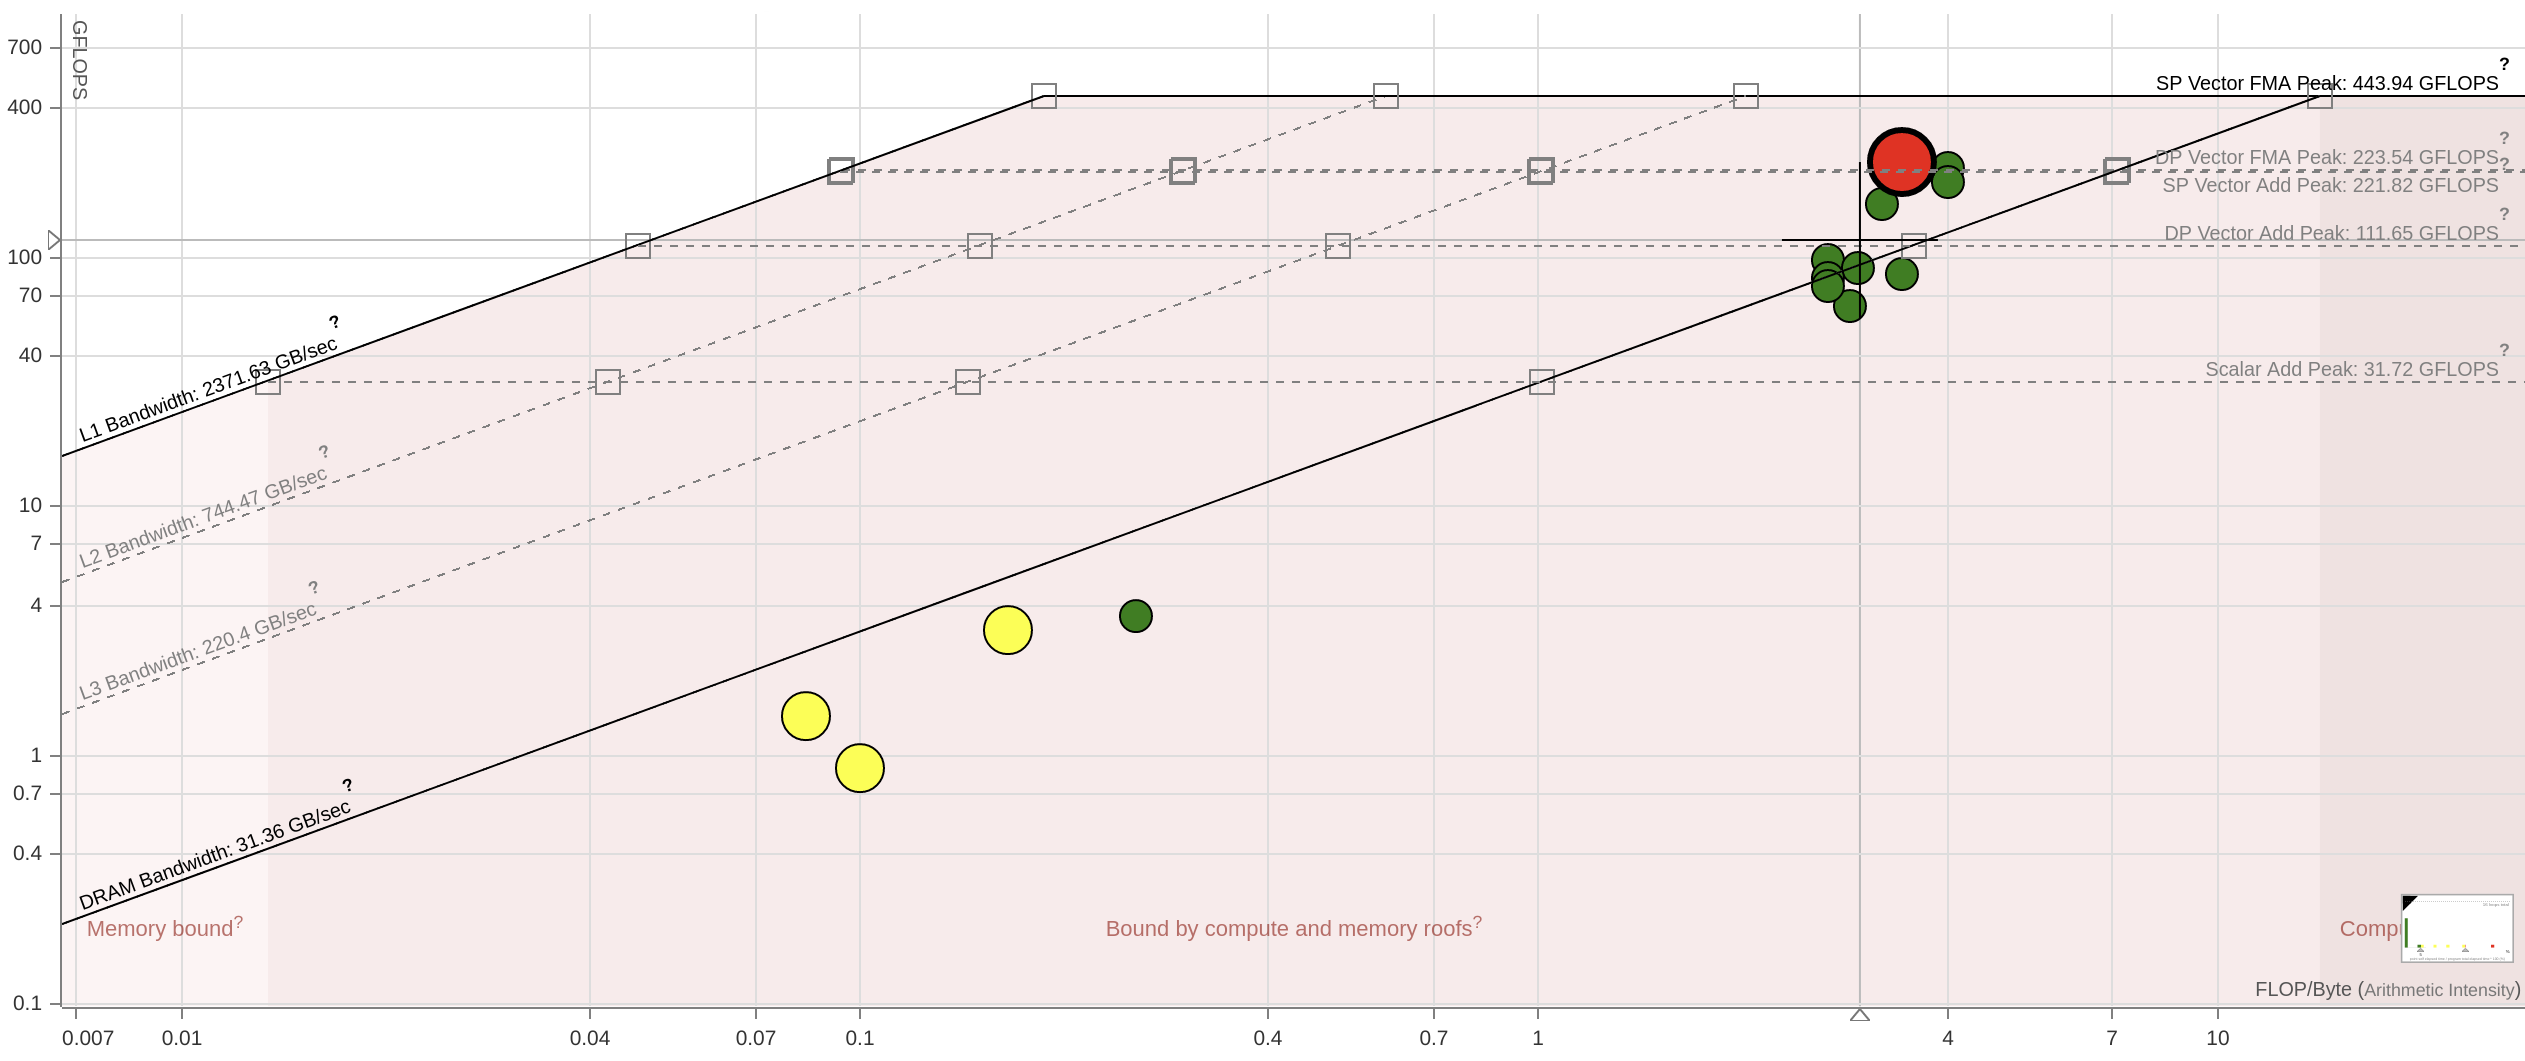
\includegraphics[width=\textwidth]{img/roofline_dense.png}
    \caption{\textit{Roofline model} del código denso}
    \label{fig:roofline_dense}
\end{figure}

Como se puede apreciar en el modelo, el \textit{workload} de interés, que es el que se puede encontrar en la parte superior derecha (coloreado en rojo y verde), corresponde a las funciones \texttt{cblas\_sgemm}. Estas funciones están fuertemente optimizadas y emplean instrucciones AVX512, como se puede observar en los detalles de la carga (Figura \ref{fig:roofline_dense_details}).

Fijándose con atención se pueden ver funciones con un considerablemente menor desempeño en la parte inferior izquierda. Estos puntos corresponden a \texttt{map\_and\_bias} y sucesivas llamadas a otras funciones como \texttt{expf}. Tal como se comenta previamente, una paralelización es sencilla de funciones auxiliares es sencilla. Sin embargo y tal como se puede ver en el modelo, se pueden distinguir perfectamente los componentes de dichas funciones, y siendo el tiempo de ejecución constante para dos redes con las mismas dimensiones, es sencillo discernir qué mejorías vienen causadas por un producto de matrices más eficiente.    

\begin{figure}[h!]
    \centering
    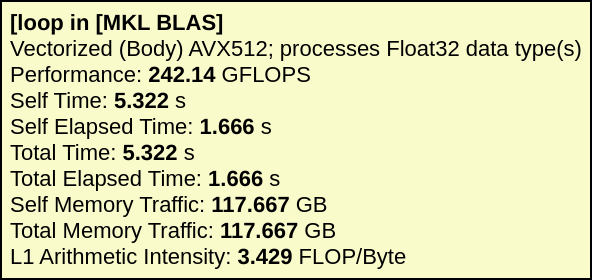
\includegraphics[width=0.5\textwidth]{img/roofline_dense_details.png}
    \caption{Detalles de \texttt{cblas\_sgemm} en el modelo del código denso}
    \label{fig:roofline_dense_details}
\end{figure}

\subsection{Código \textit{sparse}}
Por otro lado, los resultados obtenidos para la red neuronal dispersa son los siguientes:

\begin{center}
Tiempo $(\overline{t} \pm \sigma)$ = 13,862 s $\pm$ 0,710 s

Rangos (min \ldots\ max) = 12,635 s \ldots\ 15,285 s
\end{center}

En este caso, debido al empleo de la librería librsb, el modelo \textit{roofline} no contiene información de utilidad (Figura \ref{fig:roofline_sparse_details}). Esto, que a todas luces es un problema, deja de serlo si se realiza un sencillo razonamiento.

\begin{figure}[h!]
    \centering
    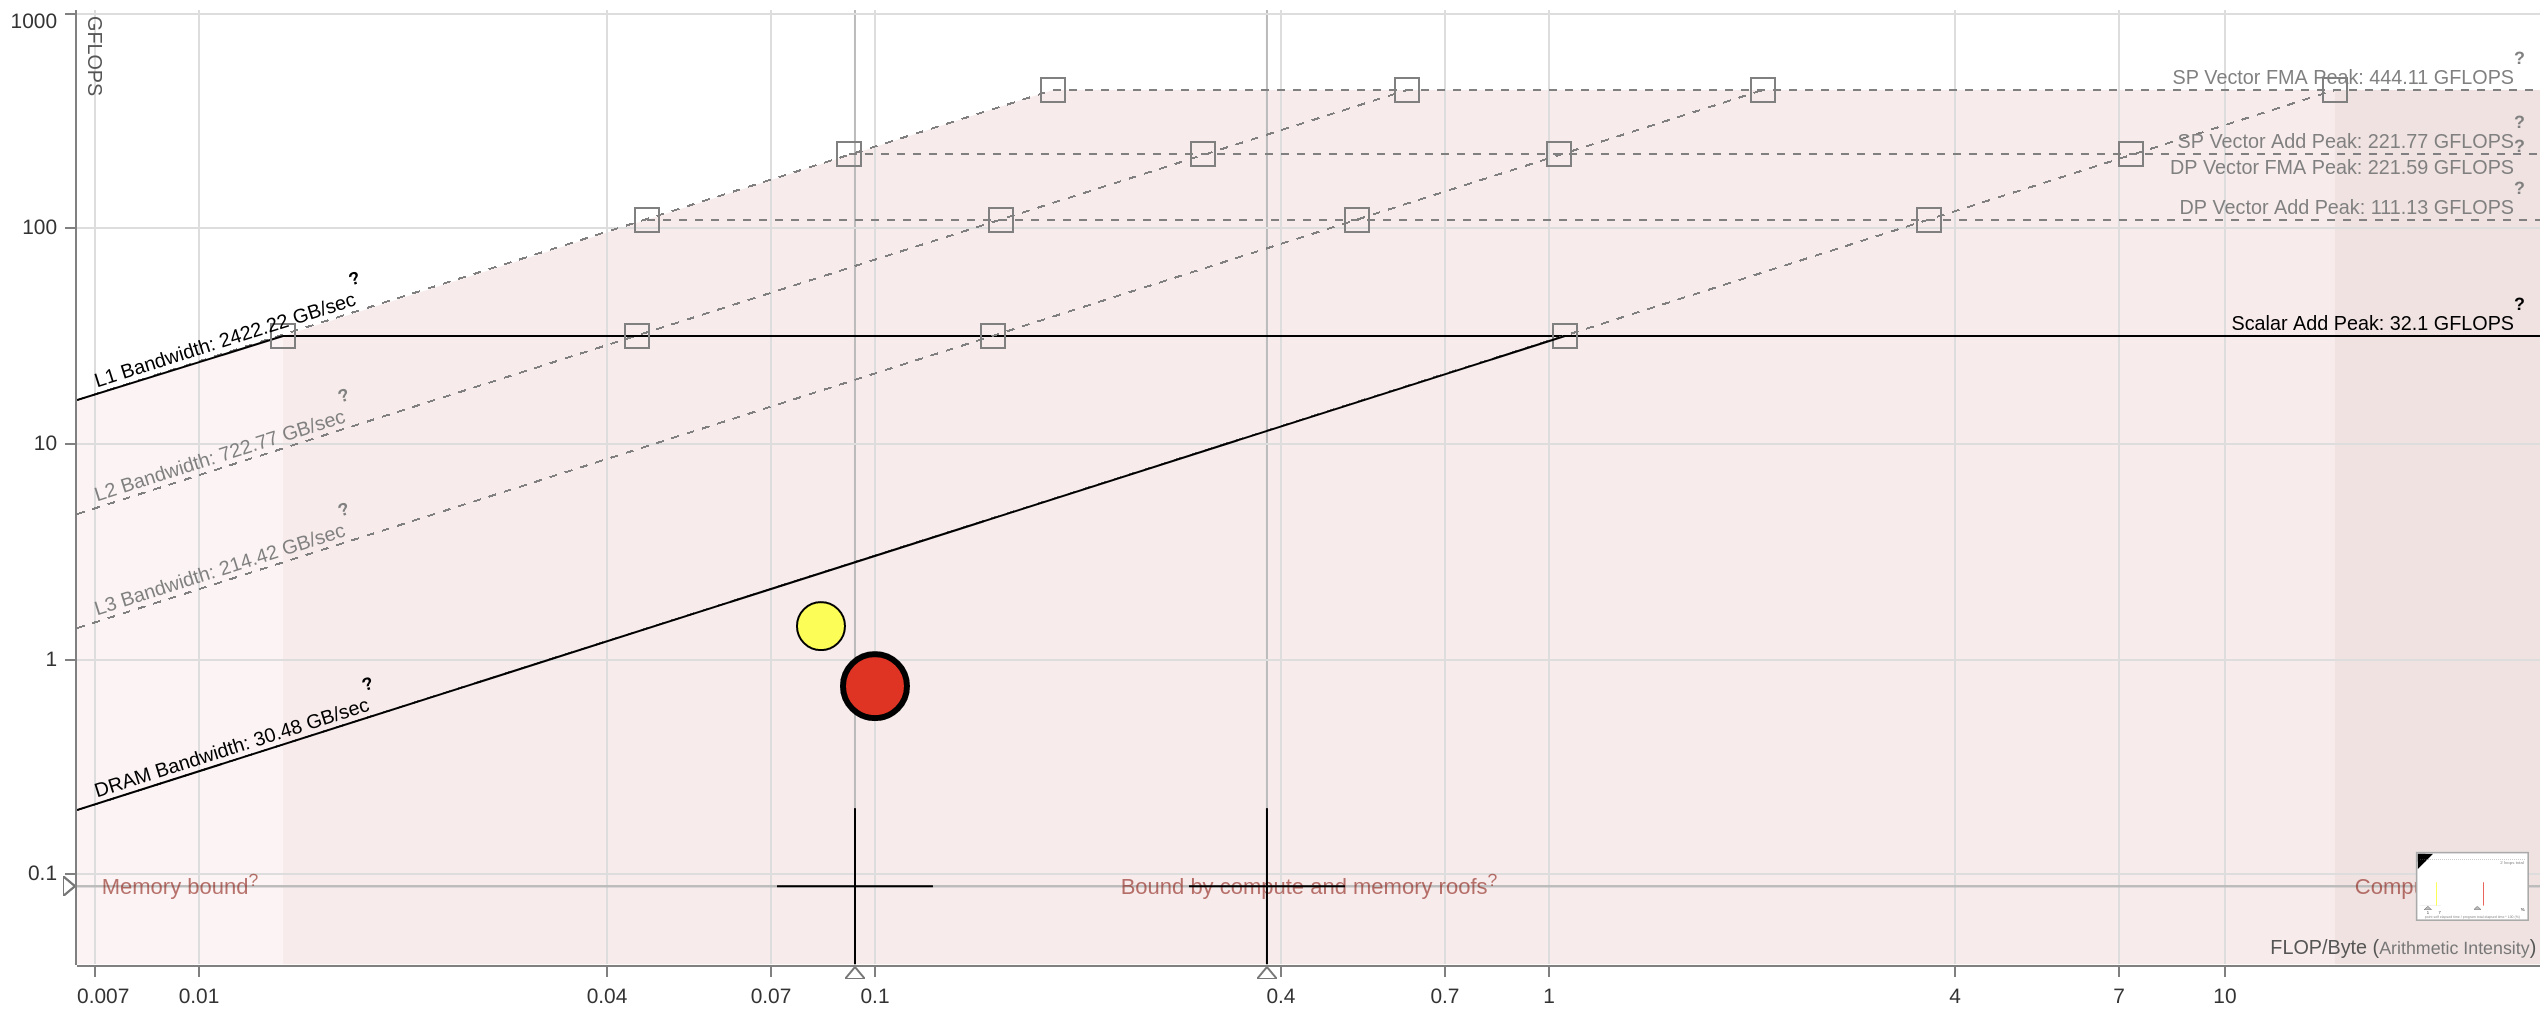
\includegraphics[width=\textwidth]{img/roofline_sparse.png}
    \caption{\textit{Roofline model} del código disperso}
    \label{fig:roofline_sparse_details}
\end{figure}

Teniendo en cuenta que los tiempos de ejecución de una red dispersa al 95\% son \textasciitilde25\% superiores a los de la red completamente conexa, aún teniendo que procesar un 95\% menos de datos, se puede realizar una estimación del número teórico de FLOP necesarios para las operaciones de multiplicación.

\subsubsection{Aproximación teórica}
Tal como se explica en la Sección \ref{sec:multiplicacion_point_to_point}, teniendo en cuenta que una operación FMA realiza dos FLOP, se puede concluir que el número de FLOP para la multiplicación de dos matrices $d\times D$ será $2 \cdot \#nz \cdot k$.

\subsubsection{Estimación del rendimiento}
Teniendo en cuenta que las matrices dispersas de pesos en el código disperso tienen una densidad del 5\% (o lo que es lo mismo, una \textit{sparsity} del 95\%), desde un punto de vista teórico se puede concluír que se deberían realizar un 95\% menos de operaciones en punto flotante.

Sin embargo esta reducción en el número de operaciones necesarias, debido a múltiples factores como el principio de localidad, estructura interna a la hora de almacenar la matriz, estructuras de control, así como optimizaciones internas de la propia librería, no se corresponde con una disminución del tiempo de ejecución, sino más bien todo lo contrario. Esta reducción en el número de FLOPS no lo es sin embargo en intensidad aritmética, puesto que también se cuenta con menor número de bytes de datos, resultando en un hipotético descenso en el eje $y$ en el modelo.

Por esta razón, el modelo \textit{roofline} resultante, que el programa Intel Advisor es incapaz de generar, se vería similar a lo que se puede observar en la Figura \ref{fig:roofline_sparse_estimado}.

\begin{figure}[h!]
    \centering
    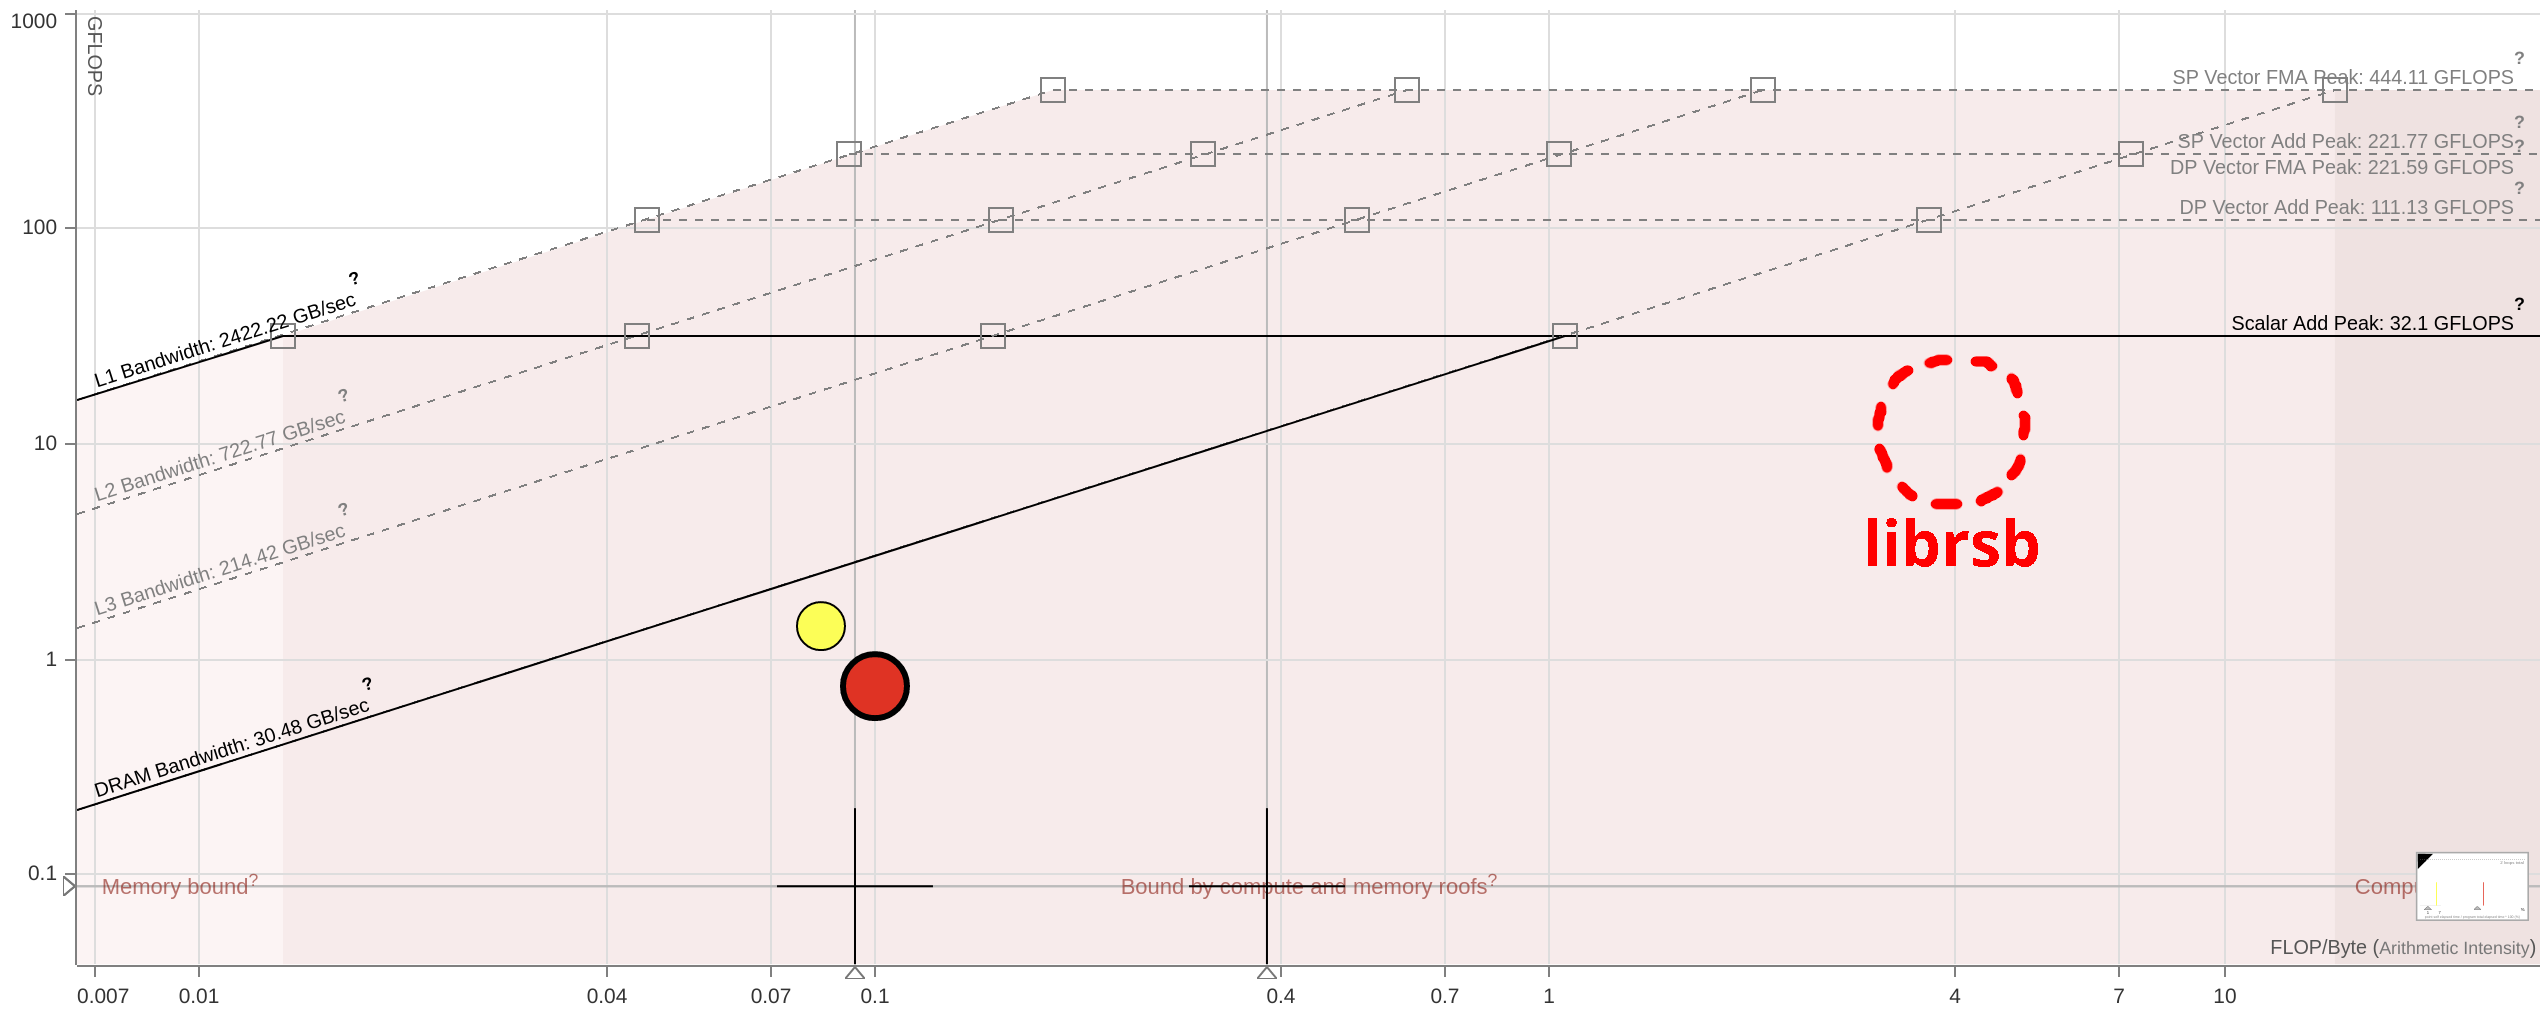
\includegraphics[width=\textwidth]{img/roofline_sparse_estimado.png}
    \caption{Estimación del \textit{roofline model} del código disperso}
    \label{fig:roofline_sparse_estimado}
\end{figure}

Estos decepcionantes resultados, sin embargo, no son tan desalentadores, ya que implica que existe un amplio margen de mejora mediante análisis estático de código y generación de instrucciones FMA y de control \textit{ad-hoc}, que incluso pueden ser vectorizadas mediante el empleo de la herramienta MARTA\footnote{\url{https://github.com/UDC-GAC/MARTA}}.
% \include{contido/aplicacion_web}
% \include{contido/planificacion_costes}
\chapter{Conclusiones}
\label{chap:conclusiones}

\lettrine{E}{n} este último capítulo se extraen las principales conclusiones de este \acrlong{tfm}, se comenta brevemente su relación con la titulación, y se tratan las líneas de investigación futuras.

\section{Conclusiones}
El objetivo principal de este trabajo ha consistido en el análisis, así como en una posible mejora de los tiempos de ejecución de modelos de inteligencia artificial en fase de inferencia y su consumo energético. Estos objetivos se han cumplido satisfactoriamente. No solamente se ha analizado en detalle el producto de matrices en este contexto, siendo este código una porción muy relevante del tiempo de ejecución de múltiples arquitecturas de redes neuronales, sino que se ha implementado de cero y en código C una red neuronal, sobre la que se han propuesto mejoras útiles bajo ciertas condiciones de \textit{sparsity}.

Los resultados obtenidos son buenos y esperanzadores, ya que mediante una paralelización sencilla, ausencia de vectorización y una ordenación de datos no necesariamente optimizada, se obtienen, a partir de aproximadamente el 87,5\% de \textit{sparsity}, tiempos de ejecución crecientemente mejores con respecto a los obtenidos por librerías \acrshort{blas} estándar en la industria. Este nivel de \textit{sparsity} es algo elevado para una red de propósito general, por lo que las optimizaciones propuestas, de momento, no pueden emplearse en la resolución de cualquier problema con un índice de dispersión más modesto. Sin embargo, tal como se puede apreciar en la Figura \ref{fig:grafica_sparse_vs_dense} (Subsección \ref{ssec:podado_y_redes_dispersas}), para una red correctamente diseñada y entrenada, es en los valores intermedios entre el 80\% y 90\% de \textit{sparsity} donde se obtiene la mejor relación entre rendimiento y precisión.

Por último, una conclusión que se puede derivar de estos resultados es en relación a la posible mejora del consumo energético de redes neuronales dispersas. Y es que resulta evidente que, como por ejemplo se comentó en la Subsección \ref{ssec:xpu}, una menor cantidad de transferencias desde memoria principal, así como una menor cantidad de operaciones en CPU, debe necesariamente traducirse en una menor cantidad de energía consumida, siempre que el diseño de la microarquitectura acompañe.

\section{Relación con la titulación}
En este trabajo se han empleado extensivamente herramientas de depuración y perfilado, tratadas principalmente en la asignatura de Herramientas para HPC. También se ha realizado una paralelización con \texttt{OpenMP} del código \textit{point-to-point}, conocimiento adquirido en las asignaturas de Programación Paralela y Programación Paralela Avanzada.

Por otro lado, el hecho de poder plantear ciertos razonamientos con respecto a la correcta utilización de la jerarquía de memoria, así como la implementación de un algoritmo optimizado para ello, no sería posible sin el trabajo realizado durante los últimos años tanto en la Especialidad de Ingeniería de Computadores del Grado en Ingeniería Informática como en este Máster en Computación de Altas Prestaciones y, más concretamente, en la asignatura de Arquitecturas de Altas Prestaciones.

\section{Trabajo futuro}
Las líneas de trabajo futuro se mencionan varias veces a lo largo de la memoria. Dado que este trabajo está orientado a futura investigación en el marco de una tesis doctoral, continuar con la optimización del código \textit{point-to-point} ha estado siempre en el horizonte cercano. Mediante el empleo de técnicas de \textit{data mining}, el uso de la herramienta MACVETH, así como mejorando la ubicación de los operandos en memoria para un mejor uso del ancho de banda de la memoria principal y la localidad caché, se espera una mejora sustancial en los rendimientos para índices de dispersión donde ya se supera a \texttt{OpenBLAS}, así como continuar expandiendo la viabilidad de esta aproximación para densidades mayores. En paralelo a estas labores de investigación y optimización de la herramienta, mejorarla para su uso por parte de otros investigadores es una prioridad, haciendo así que deje de ser una simple Prueba de Concepto. Esto se realizaría en varios pasos: 
\begin{itemize}
    \item Conversión del \textit{Jupyter Notebook} a una herramienta universal, programada en Python de inicio a fin, que lea una red neuronal como entrada y genere código como salida. Esta herramienta podría ser tanto interactiva como no interactiva.
    \item Mejora en la modularización de la herramienta y generación de código. Ahora mismo los \textit{backends} implementados son lentos, y poco mantenibles, por lo que necesitarían una puesta a punto. Además, es conveniente dividir el código en varias secciones lógicas, para poder realizar la compilación y optimización en diversas \textit{translation units}\footnote{\url{https://en.wikipedia.org/wiki/Translation_unit_(programming)}}, y así aprovechar los múltiples núcleos que ofrece un procesador moderno.
    \item Implementar un mecanismo automatizado sobre la herramienta, de tal forma que se pueda seguir un \textit{workflow} ágil, pudiéndole suministrar enlaces a redes en formato \textit{ONNX} para la conversión a uno o más ficheros C, que sean analizados, optimizados y compilados.
    \item Mejora en la obtención de métricas, particularmente en el actual sistema de medición de tiempos integrando, por ejemplo, un sistema de medición de contadores PAPI.
    \item Implementación de otros \textit{backends} tanto para arquitecturas ya existentes como para arquitecturas \textit{ad hoc}, por ejemplo, en ensamblador o VHDL.
    \item Implementación de soporte para memoria distribuida mediante MPI\footnote{\url{https://www.mpi-forum.org/docs/}}.
\end{itemize}


%%%%%%%%%%%%%%%%%%%%%%%%%%%%%%%%%%%%%%%%
% Apéndices, glosarios e bibliografía  %
%%%%%%%%%%%%%%%%%%%%%%%%%%%%%%%%%%%%%%%%

% \appendix
% \appendixpage
% \include{anexos/factsheet_europe}
% \include{anexos/bench_values}
% \include{anexos/archlinux_maintenance_guide}

% \printglossary[type=\acronymtype,title=\nomeglosarioacronimos]
% \printglossary[title=\nomeglosariotermos]

\bibliographystyle{IEEEtranN}
\bibliography{\bibconfig,bibliografia/bibliografia}
\cleardoublepage

\end{document}

%%%%%%%%%%%%%%%%%%%%%%%%%%%%%%%%%%%%%%%%%%%%%%%%%%%%%%%%%%%%%%%%%%%%%%%%%%%%%%%%
